\documentclass[12pt,a4paper]{report}
\usepackage{pre-tese}
\makeindex

% Logo da Escola de Engenharia
\logo{EE}{Escola de Engenharia}{}
\logoB{EE}{Escola de Engenharia}{}

\author{Diogo André da Silva Esteves}

\titleA{Otimização e Padronização}
\titleB{de Processos de Gestão}
\titleC{Medicamentosa em Ambiente Hospitalar}

\masters{Mestrado em Engenharia Bioinformática}
% ATUALIZAR: Inserir nome real do orientador
\supervisor{Prof. Dr. José Manuel Ferreira Machado}
% ATUALIZAR: Inserir nome real do coorientador (opcional)
\cosupervisor{Prof. Dr. Ana Regina Coelho de Sousa}

\bibpunct[,]{(}{)}{;}{a}{,}{,}
\begin{document}
\setlength{\parindent}{0em}

%-- Covers
% Front Cover - Seguindo template oficial UMinho
\begin{titlepage}

% Logos UMinho e Escola de Engenharia - centralizado conforme template
\begin{center}
\thelogo
\end{center}

% Título - mais compactado
\vspace*{10mm}
\begin{center}
    {\huge\bfseries \thetitleA}
    \vspace{3mm}
    {\huge\bfseries \thetitleB}
    \vspace{3mm}
    {\huge\bfseries \thetitleC}
\end{center}

% Grau e área - mais compactado
\vspace{10mm}
\begin{center}
    {\Large \themasters}
\end{center}

% Autor - mais compactado
\vspace{8mm}
\begin{center}
    {\large \theauthor}
\end{center}

% Orientação - mais compactado
\vspace{10mm}
\begin{center}
    {\footnotesize Trabalho efetuado sob a orientação de\\
    \vspace{2mm}
    \textbf{\thesupervisor}}
    \ifthenelse{\equal{\thecosupervisor}{}}{}{\\
    \vspace{2mm}
    e coorientação de\\
    \vspace{2mm}
    \textbf{\thecosupervisor}}
\end{center}

% Local e data - compactado para caber na primeira página
\vspace{15mm}
\begin{center}
    {\large Universidade do Minho, Escola de Engenharia, \myear}
\end{center}

\end{titlepage}

% Página em branco para pré-tese
\newpage
\thispagestyle{empty}
\mbox{} 

%-- Document setup
\newgeometry{right=25mm, left=25mm, top=25mm, bottom=25mm}
\pagenumbering{roman}

\setlength{\parskip}{0pt}
\setlength{\parindent}{1.5em}

%-- Preamble
\chapter*{Resumo}
\addcontentsline{toc}{chapter}{Resumo}

A fragmentação dos sistemas de informação no Serviço Nacional de Saúde português representa um desafio sistémico à segurança do doente e à eficiência operacional, particularmente no ciclo do medicamento. Este projeto de dissertação propõe-se a endereçar este problema no contexto da Santa Casa da Misericórdia de Vila Verde (SCMVV) através do desenho, desenvolvimento e avaliação de uma plataforma de software centralizada. O objetivo é unificar os fluxos de trabalho clínico-farmacêuticos, atualmente dispersos por múltiplos sistemas legados, numa única interface de utilizador moderna e coesa.

Adotando uma metodologia de \textit{Design Science Research} (DSR), o projeto irá criar um artefacto tecnológico — um sistema web com uma arquitetura de microsserviços (Node.js) e um frontend reativo (TypeScript/React) — concebido para se integrar com a infraestrutura existente. A avaliação do sistema será focada em indicadores de desempenho chave (KPIs) específicos, antecipando-se uma redução significativa dos erros de medicação e um aumento da eficiência dos processos para enfermeiros e farmacêuticos. A contribuição principal deste trabalho será a validação de um modelo de modernização sociotécnica que, se bem-sucedido, poderá servir de referência para outras unidades de saúde que enfrentam desafios de fragmentação semelhantes.

\vspace{6mm}
\noindent\textbf{Palavras-chave:} Sistemas de Informação em Saúde, Segurança do Doente, Gestão da Medicação, Design Science Research, Unificação de Sistemas, Interoperabilidade Clínica.

\vspace*{\fill}

\chapter*{Abstract}
\addcontentsline{toc}{chapter}{Abstract}

The fragmentation of information systems within the Portuguese National Health Service constitutes a systemic challenge to patient safety and operational efficiency, particularly in the medication management lifecycle. This dissertation project aims to address this problem in the context of the Santa Casa da Misericórdia de Vila Verde (SCMVV) by designing, developing, and evaluating a centralized software platform. The primary objective is to unify the clinical-pharmaceutical workflows, currently fragmented across multiple legacy systems, into a single, modern, and cohesive user interface.

Adopting a \textit{Design Science Research} (DSR) methodology, the project will create a technological artifact—a web-based system featuring a microservices architecture (Node.js) and a reactive frontend (TypeScript/React)—designed to integrate with the existing infrastructure. The system's evaluation will focus on specific Key Performance Indicators (KPIs), with the anticipation of achieving a significant reduction in medication errors and an increase in process efficiency for nurses and pharmacists. The main contribution of this work will be the validation of a sociotechnical modernization model that, if successful, could serve as a reference for other healthcare institutions facing similar fragmentation challenges.

\vspace{6mm}
\noindent\textbf{Keywords:} Health Information Systems, Patient Safety, Medication Management, Design Science Research, System Unification, Clinical Interoperability. 
\chapter*{Agradecimentos}
\addcontentsline{toc}{chapter}{Agradecimentos}

Gostaria de expressar os meus sinceros agradecimentos a todas as pessoas e instituições que tornaram possível a realização deste trabalho.

Em primeiro lugar, ao meu orientador Prof. Dr. José Machado, pela orientação científica, apoio metodológico e conhecimento partilhado ao longo de todo o processo de investigação. A sua experiência na área de sistemas de informação em saúde foi fundamental para o desenvolvimento deste projeto.

Ao meu coorientador Profa. Dra. Regina Sousa, pelas valiosas contribuições técnicas e perspetivas que enriqueceram significativamente este trabalho, especialmente na área de arquitetura de software e integração de sistemas.

Ao Prof. Dr. Antonio Abelha, pela orientação em contexto clínico e pela disponibilidade para partilhar o seu conhecimento e experiência no domínio da gestão medicamentosa hospitalar e na sua analise de dados com queries SQL quase cirúrgicas para o problema apresentado.

À Universidade do Minho e à Escola de Engenharia, por proporcionarem as condições necessárias para a realização desta investigação, incluindo o acesso a recursos computacionais e bibliográficos essenciais.

À administração e profissionais de saúde do Hospital da Misericórdia de Vila Verde (SCMVV), pela colaboração e disponibilidade para partilhar o seu conhecimento e experiência no domínio da gestão hospitalar e do sistema em produção.

Aos técnicos de sistemas de informação da SCMVV, pela assistência técnica e acesso aos sistemas legados, que permitiu a compreensão detalhada dos processos existentes.

Aos meus colegas do Mestrado em Engenharia Bioinformática, pelo companheirismo, discussões enriquecedoras e partilha de conhecimentos que contribuíram para o enriquecimento académico.

À minha família, pelo apoio incondicional, compreensão e incentivo durante todo o percurso académico, especialmente nos momentos mais desafiantes.

A todos os que, direta ou indiretamente, contribuíram para a realização deste trabalho, o meu profundo agradecimento.

\cleardoublepage 

%-- Lista de Abreviaturas e Símbolos
\chapter*{Lista de Abreviaturas e Símbolos}
\addcontentsline{toc}{chapter}{Lista de Abreviaturas e Símbolos}

\begin{description}
\item[API] Application Programming Interface
\item[CDSS] Clinical Decision Support System
\item[CPOE] Computerized Physician Order Entry
\item[EHR] Electronic Health Record
\item[FHIR] Fast Healthcare Interoperability Resources
\item[HL7] Health Level Seven
\item[HIS] Hospital Information System
\item[JWT] JSON Web Token
\item[KPI] Key Performance Indicator
\item[ML] Machine Learning
\item[NLP] Natural Language Processing
\item[RGPD] Regulamento Geral sobre a Proteção de Dados
\item[ROI] Return on Investment
\item[SCMVV] Santa Casa da Misericórdia de Vila Verde
\item[SGBD] Sistema de Gestão de Base de Dados
\item[SSO] Single Sign-On
\item[TAM] Technology Acceptance Model
\item[UI] User Interface
\item[UX] User Experience
\end{description}

\cleardoublepage

%-- Índices
\phantomsection
\addcontentsline{toc}{chapter}{Índice}
\tableofcontents

\cleardoublepage
\phantomsection
\addcontentsline{toc}{chapter}{Lista de Figuras}
\listoffigures

\cleardoublepage
\phantomsection
\addcontentsline{toc}{chapter}{Lista de Tabelas}
\listoftables

\cleardoublepage
\pagenumbering{arabic}

%-- Capítulos da Pré-Tese
\chapter{Introdução}

% [NOTA: Remover parágrafo redundante - esta informação já aparece nos objetivos]
A gestão medicamentosa em ambiente hospitalar constitui um dos processos mais críticos e complexos das instituições de saúde modernas. O Hospital da Misericórdia de Vila Verde (SCMVV), à semelhança de outras unidades hospitalares nacionais, enfrenta desafios significativos na coordenação entre prescrição médica, validação farmacêutica e administração por enfermagem. Este trabalho apresenta o desenvolvimento e implementação de um sistema integrado de gestão medicamentosa que visa resolver estas lacunas através de tecnologias modernas.

\section{Contexto e Enquadramento}

A gestão medicamentosa em ambiente hospitalar constitui um dos processos mais críticos e complexos do sistema de saúde \cite{kohn2000,berwick2008}. No Hospital da Santa Casa da Misericórdia de Vila Verde (SCMVV), a necessidade de modernização dos sistemas informáticos tornou-se evidente face aos desafios crescentes de segurança, eficiência e rastreabilidade.

\begin{figure}[htbp]
    \centering
    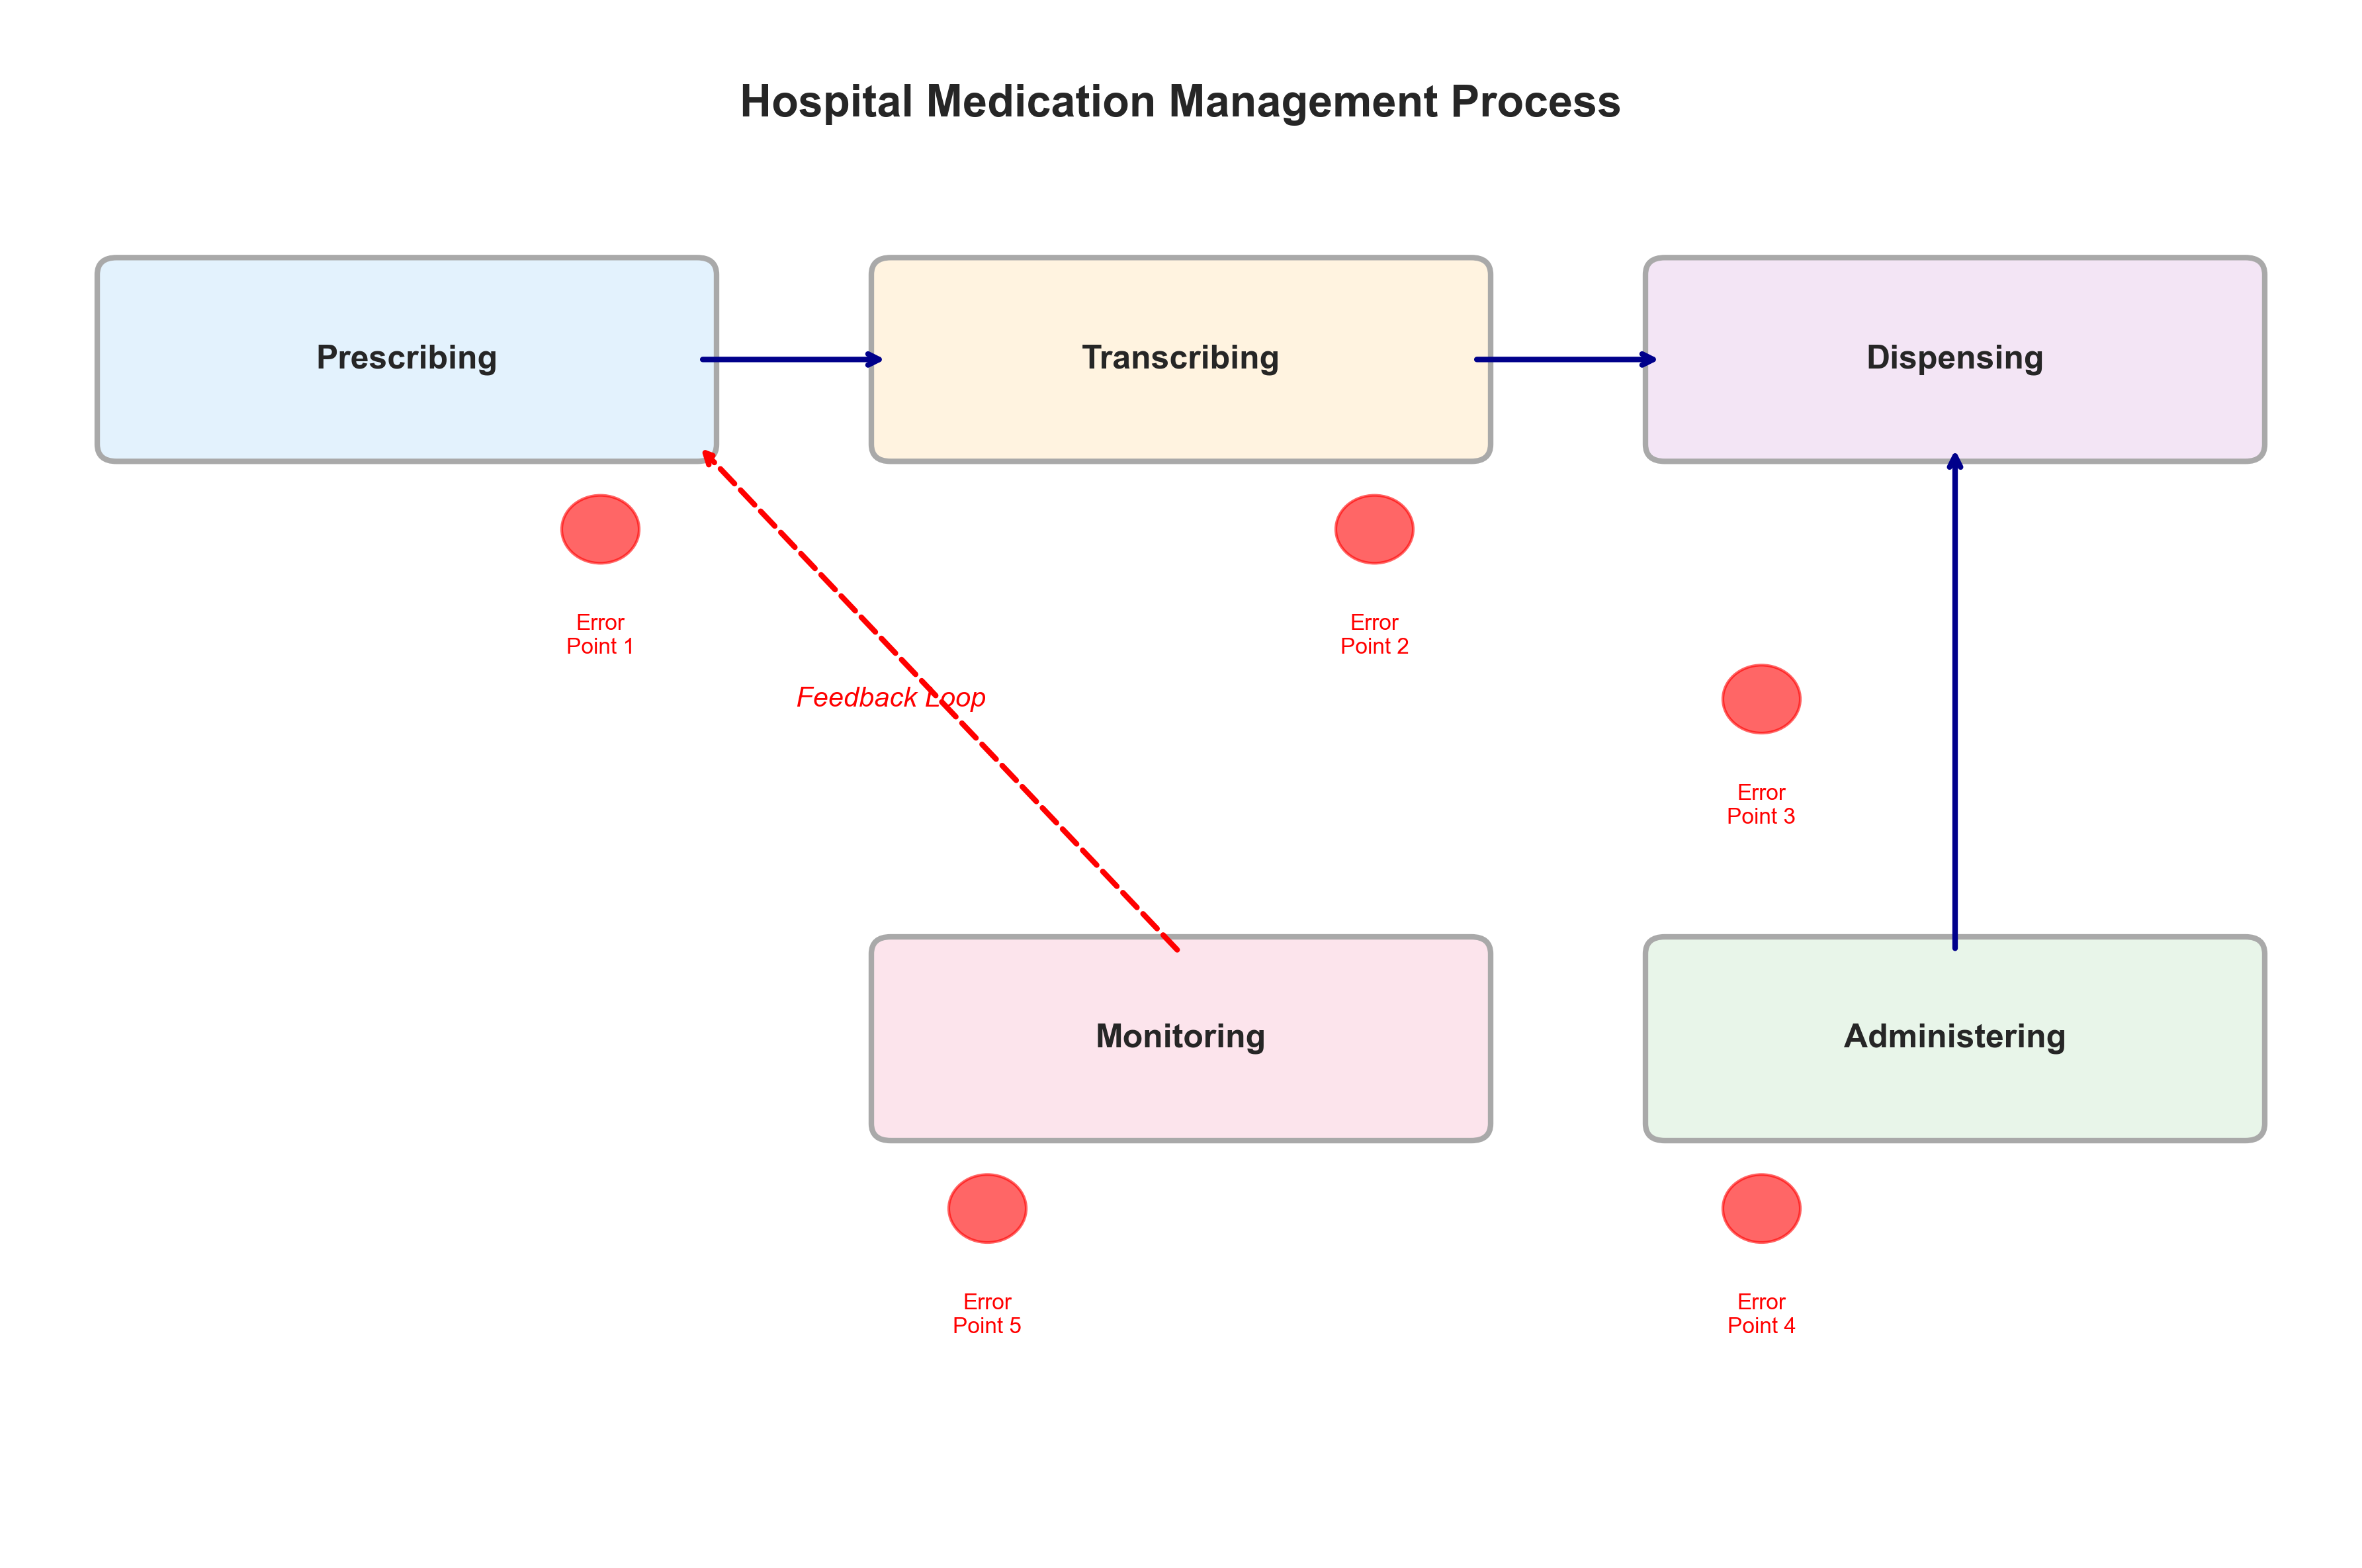
\includegraphics[width=0.9\textwidth]{images/generated/medication_flow_process.png}
    \caption{Hospital medication management process showing the five main stages and potential error points. Adapted from the medication use process framework \citep{austin2018,zheng2021}.}
    \label{fig:medication_flow}
\end{figure}

Os sistemas hospitalares portugueses operam frequentemente com soluções fragmentadas, desenvolvidas em diferentes épocas \cite{kazemi2016} e com tecnologias díspares. Na SCMVV, o sistema legado AIDA-PCE, implementado antes de 2010, continua operacional mas apresenta limitações significativas:

O sistema apresenta uma interface desatualizada que dificulta a navegação e aumenta significativamente o tempo necessário para prescrição médica. A ausência de validações automáticas em tempo real \cite{moss2015} compromete a segurança do paciente, enquanto a falta de integração com sistemas modernos de gestão hospitalar resulta em silos de informação e processos fragmentados. 

Adicionalmente, as dificuldades na geração de relatórios e análise de dados \cite{bowles2020} limitam a capacidade de monitorização e melhoria contínua. Os problemas de escalabilidade com o aumento do volume de pacientes evidenciam a necessidade urgente de modernização tecnológica.

% [INSERIR: Tabela 1.1 - Estatísticas de erros de medicação em hospitais portugueses (fonte: DGS)]

\section{Motivação e Relevância}

Segundo dados da Organização Mundial de Saúde \cite{who2017,who2022}, os erros de medicação afetam 1 em cada 10 pacientes \cite{who2017} hospitalizados globalmente. Em Portugal, embora não existam estatísticas oficiais consolidadas, estima-se que o impacto seja similar \cite{dgs2020}. A implementação de sistemas integrados de gestão medicamentosa \cite{shermock2023,vaghasiya2023} pode reduzir estes erros em até 85\% \cite{mahoney2007}.

% [DESENVOLVER: Adicionar dados específicos da SCMVV - número de camas, prescrições/dia, etc.]

\section{Objetivos}

\subsection{Objetivo Geral}
Desenvolver um sistema integrado de gestão medicamentosa que otimize os processos de prescrição, validação, dispensa e administração de medicamentos na SCMVV, garantindo maior segurança do paciente \cite{ciapponi2021} e eficiência operacional.

\subsection{Objetivos Específicos}

Para alcançar o objetivo geral, foram definidos cinco objetivos específicos fundamentais. Primeiro, modernizar a interface do sistema através do desenvolvimento de uma interface intuitiva e responsiva utilizando React \cite{misra2023} e Material-UI, com o objetivo de reduzir o tempo médio de prescrição. Segundo, implementar um sistema robusto de validação em tempo real para interações medicamentosas \cite{moss2015,belle2013} e dosagens, aumentando a segurança do paciente.

Terceiro, garantir rastreabilidade completa através do estabelecimento de auditoria abrangente de todas as operações \cite{european2016}, permitindo monitorização e análise retrospetiva. Quarto, integrar o sistema com SONHO, farmácia e outros sistemas hospitalares através de APIs RESTful \cite{mandl2020}, eliminando silos de informação. Finalmente, otimizar a performance do sistema através de técnicas avançadas de caching e otimização de queries Oracle \cite{jiang2014}.

\section{Contribuições do Trabalho}

Este trabalho apresenta contribuições significativas para o campo da gestão medicamentosa hospitalar. A principal contribuição técnica consiste numa arquitetura modular baseada em microserviços \cite{newman2021} que permite evolução independente de componentes, facilitando manutenção e extensibilidade futura. 

O desenvolvimento de um sistema de validação inteligente representa uma contribuição importante, implementando um motor de regras extensível para validação de prescrições \cite{amland2019} que pode ser adaptado a diferentes contextos hospitalares. A consolidação de múltiplos sistemas numa interface unificada \cite{bowles2020} constitui uma contribuição prática que melhora significativamente a experiência do utilizador.

Do ponto de vista técnico, o modelo de dados otimizado proporciona uma estrutura eficiente para consultas complexas em Oracle \cite{lin2018}, enquanto o framework de testes desenvolvido garante qualidade e confiabilidade através de uma suite completa de validações \cite{martin2017}.

% [INSERIR: Figura 1.2 - Arquitetura geral da solução proposta]

\section{Estrutura da Dissertação}

% [NOTA: Simplificar - remover descrições óbvias]
Os capítulos seguintes desenvolvem o trabalho realizado:
\textbf{Capítulo 2} apresenta o estado da arte;
\textbf{Capítulo 3} detalha o plano de trabalho;
\textbf{Capítulo 4} descreve a metodologia;
\textbf{Capítulo 5} apresenta os resultados;
\textbf{Capítulo 6} discute as implicações;
\textbf{Capítulo 7} conclui com trabalho futuro. 
\chapter{Estado da Arte}

% [NOTA: Adicionar citações bibliográficas em todo o capítulo]

\section{Sistemas de Gestão Medicamentosa Hospitalar}

\subsection{Evolução Histórica}

Os sistemas de informação hospitalar (HIS) evoluíram significativamente desde os primeiros sistemas baseados em mainframes dos anos 1960. A transição para sistemas departamentais nos anos 1980 e a posterior integração através de Health Level Seven (HL7) \cite{dolin2006,mandl2020} nos anos 1990 estabeleceram as bases para os sistemas modernos.

\begin{figure}[htbp]
    \centering
    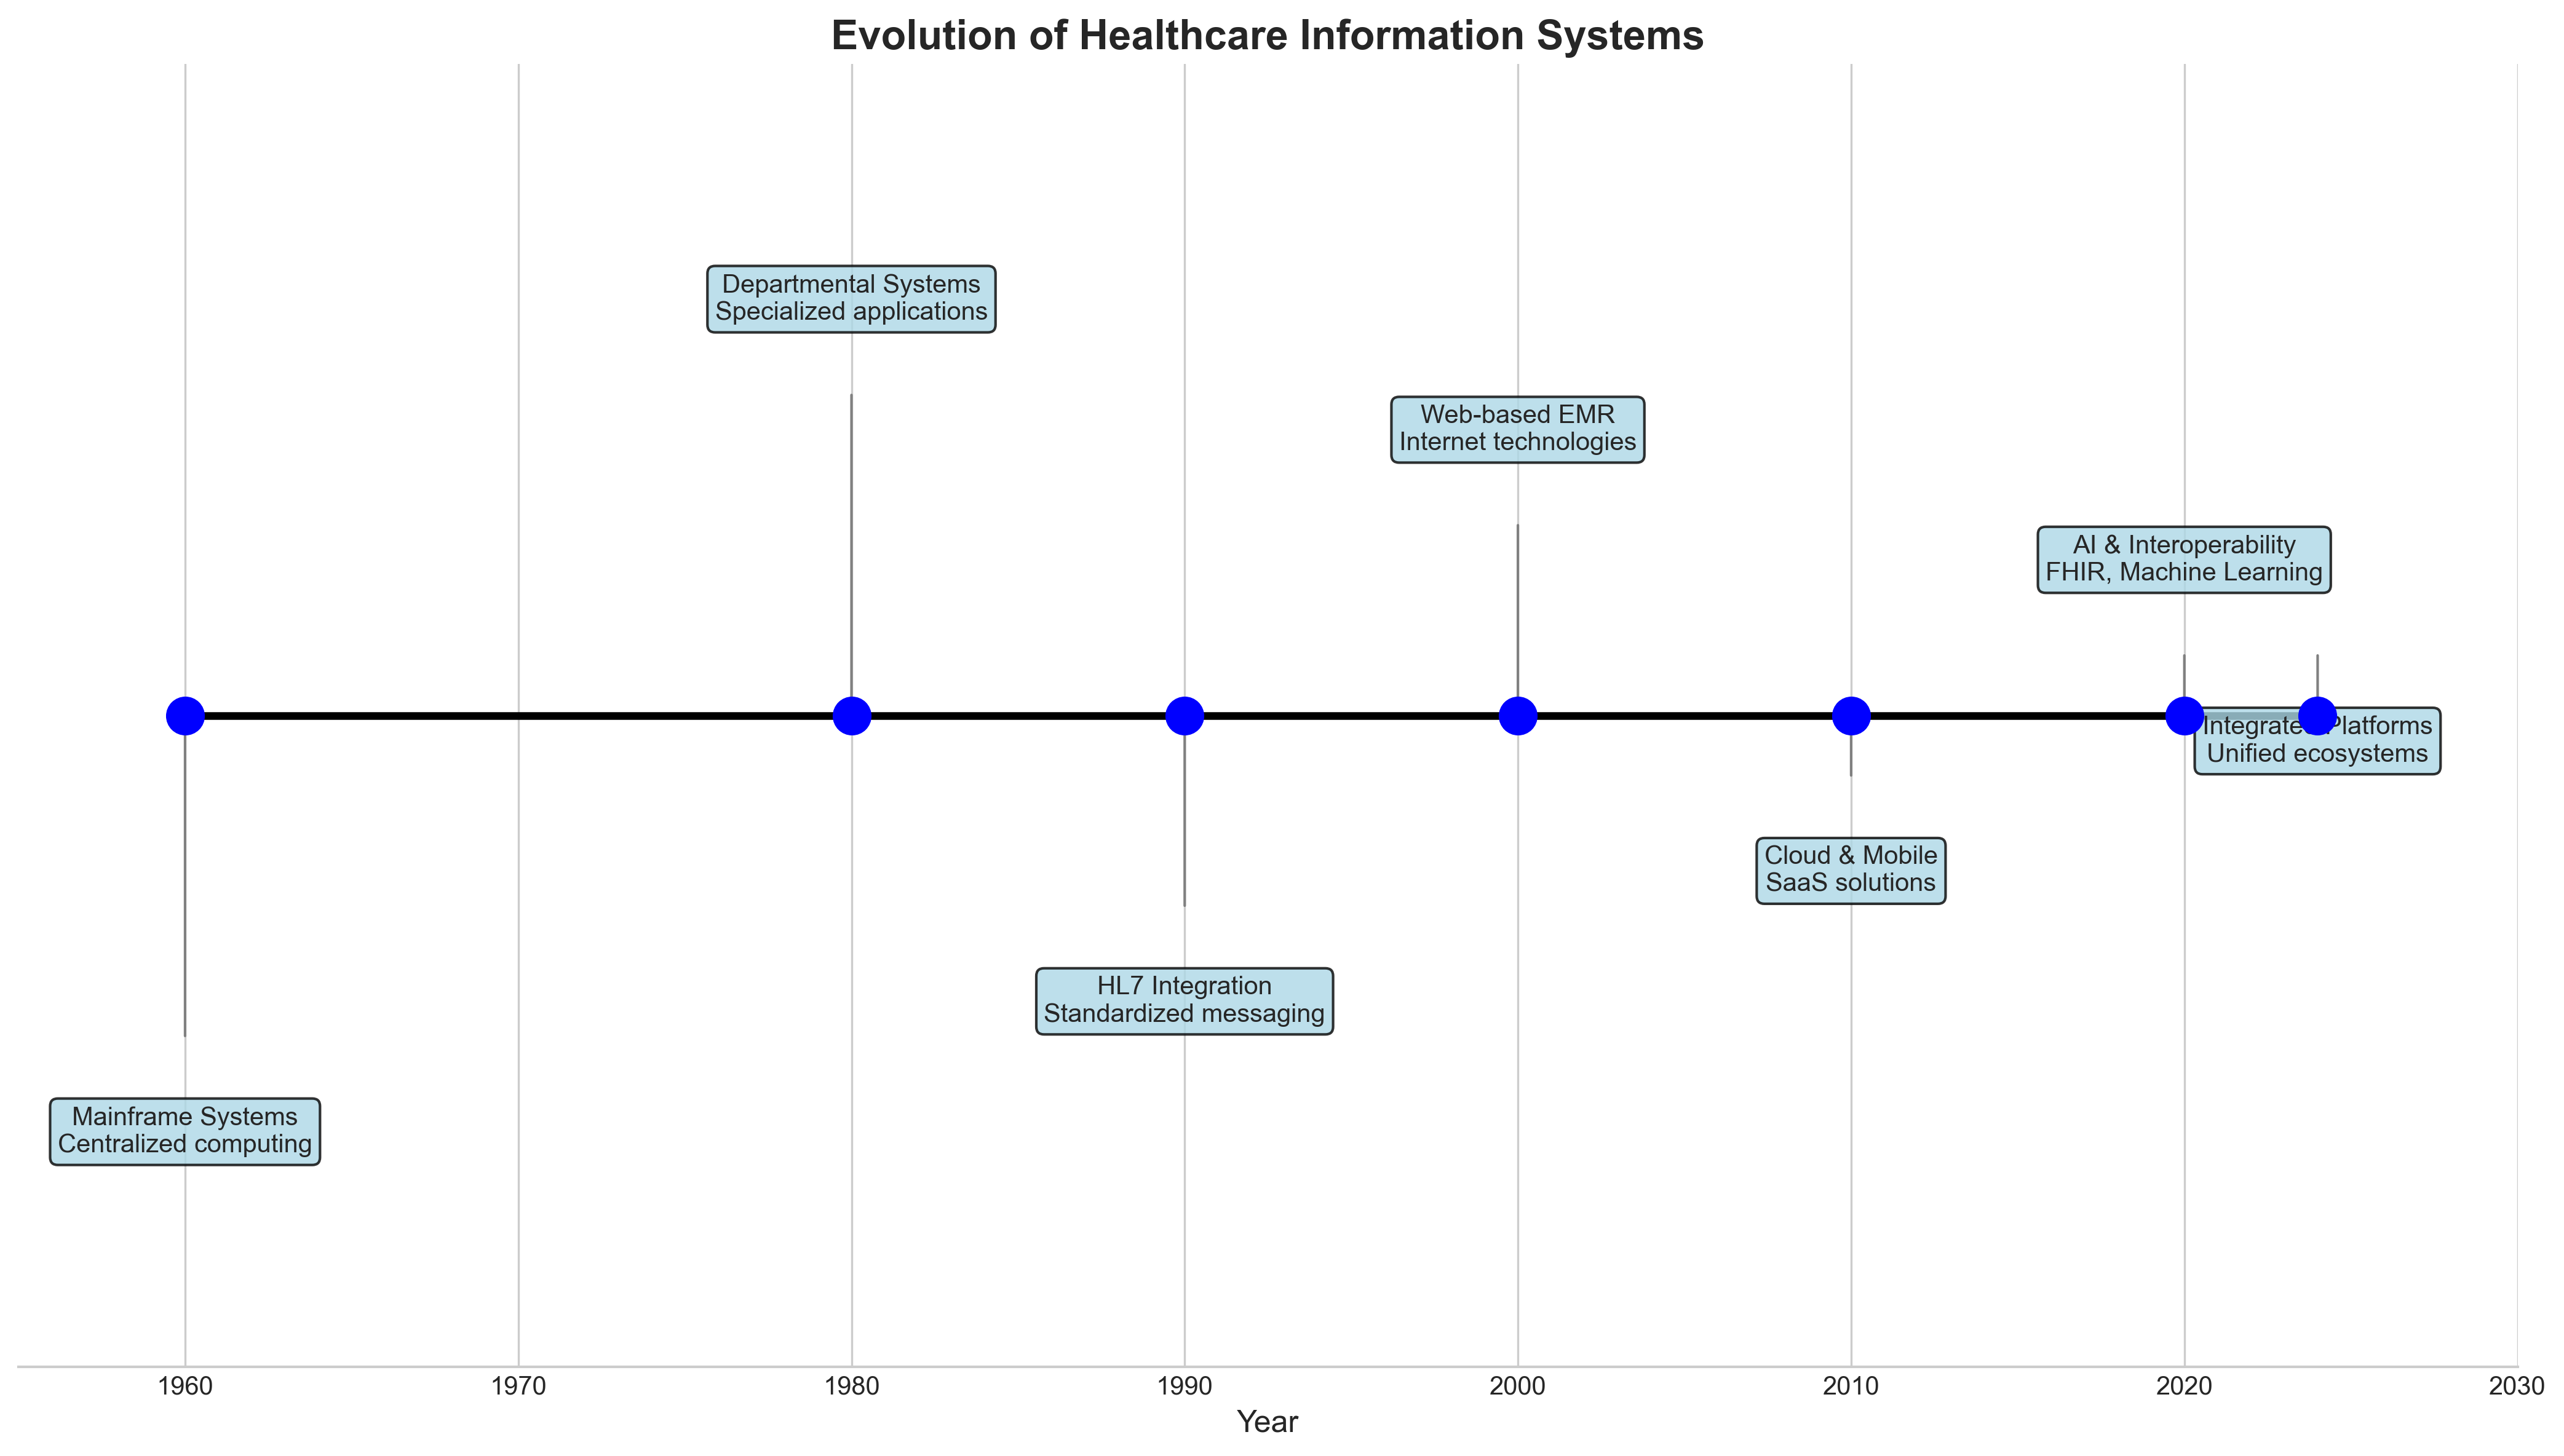
\includegraphics[width=0.95\textwidth]{images/generated/healthcare_it_timeline.png}
    \caption{Evolution of healthcare information systems from mainframe to integrated platforms \citep{shermock2023,vaghasiya2023}.}
    \label{fig:timeline}
\end{figure}

\subsection{Sistemas Comerciais Atuais}

O panorama atual dos sistemas comerciais de gestão hospitalar é dominado por alguns fornecedores principais. A Epic Systems \cite{hertzum2022} estabeleceu-se como líder de mercado nos Estados Unidos com o seu sistema EpicCare, oferecendo uma plataforma integrada para gestão clínica e administrativa. A Cerner, recentemente adquirida pela Oracle Health \cite{lin2018}, compete diretamente com as suas soluções PowerChart e Millennium, particularmente populares em hospitais de média e grande dimensão.

No mercado europeu, destaca-se a InterSystems com o TrakCare, que ganhou aceitação significativa devido à sua capacidade de adaptação a diferentes contextos regulamentares. A Allscripts, com o Sunrise Clinical Manager, mantém uma posição relevante especialmente em hospitais que procuram soluções mais flexíveis e personalizáveis.

% [INSERIR: Tabela 2.1 - Comparação de funcionalidades dos principais sistemas]

\subsection{Desafios dos Sistemas Atuais}

Apesar dos avanços tecnológicos, os sistemas atuais enfrentam desafios significativos que limitam a sua eficácia. A interoperabilidade limitada \cite{keasberry2017} representa um obstáculo major, com a falta de standards efetivos a impedir a comunicação seamless entre diferentes sistemas hospitalares. Esta fragmentação resulta em silos de informação que comprometem a continuidade de cuidados.

A complexidade das interfaces \cite{mcgreevey2020} constitui outro desafio crítico, frequentemente causando fadiga de alertas nos profissionais de saúde. Os custos elevados \cite{adler2021} de implementação e manutenção representam uma barreira significativa, especialmente para hospitais de menor dimensão. Finalmente, a resistência à mudança \cite{holden2011,venkatesh2003} permanece um fator limitante, refletindo a importância dos fatores humanos e organizacionais na adoção de novas tecnologias.

\section{Segurança na Medicação}

% [DESENVOLVER: Adicionar estatísticas europeias e nacionais]

Os erros de medicação \cite{ciapponi2021,mulac2020} constituem uma das principais causas de eventos adversos evitáveis:
- Globalmente: 1 em 10 pacientes afetados (OMS, 2022)
- Europa: 8-12\% das admissões hospitalares % [CITAR: European Commission Report \cite{european2016}]
- Portugal: Dados limitados mas estimativas similares \cite{dgs2020} % [CONTACTAR: DGS para dados oficiais]

\subsection{Tipos de Erros Mais Frequentes}

\begin{enumerate}
    \item \textbf{Erros de prescrição} (30-40\%): Dose incorreta, medicamento errado \cite{isaacs2021}
    \item \textbf{Erros de transcrição} (12-20\%): Interpretação incorreta \cite{manias2021}
    \item \textbf{Erros de dispensa} (11-15\%): Troca de medicamentos \cite{kallio2020}
    \item \textbf{Erros de administração} (26-38\%): Via, horário ou paciente errado \cite{boytim2018}
\end{enumerate}

\begin{figure}[htbp]
    \centering
    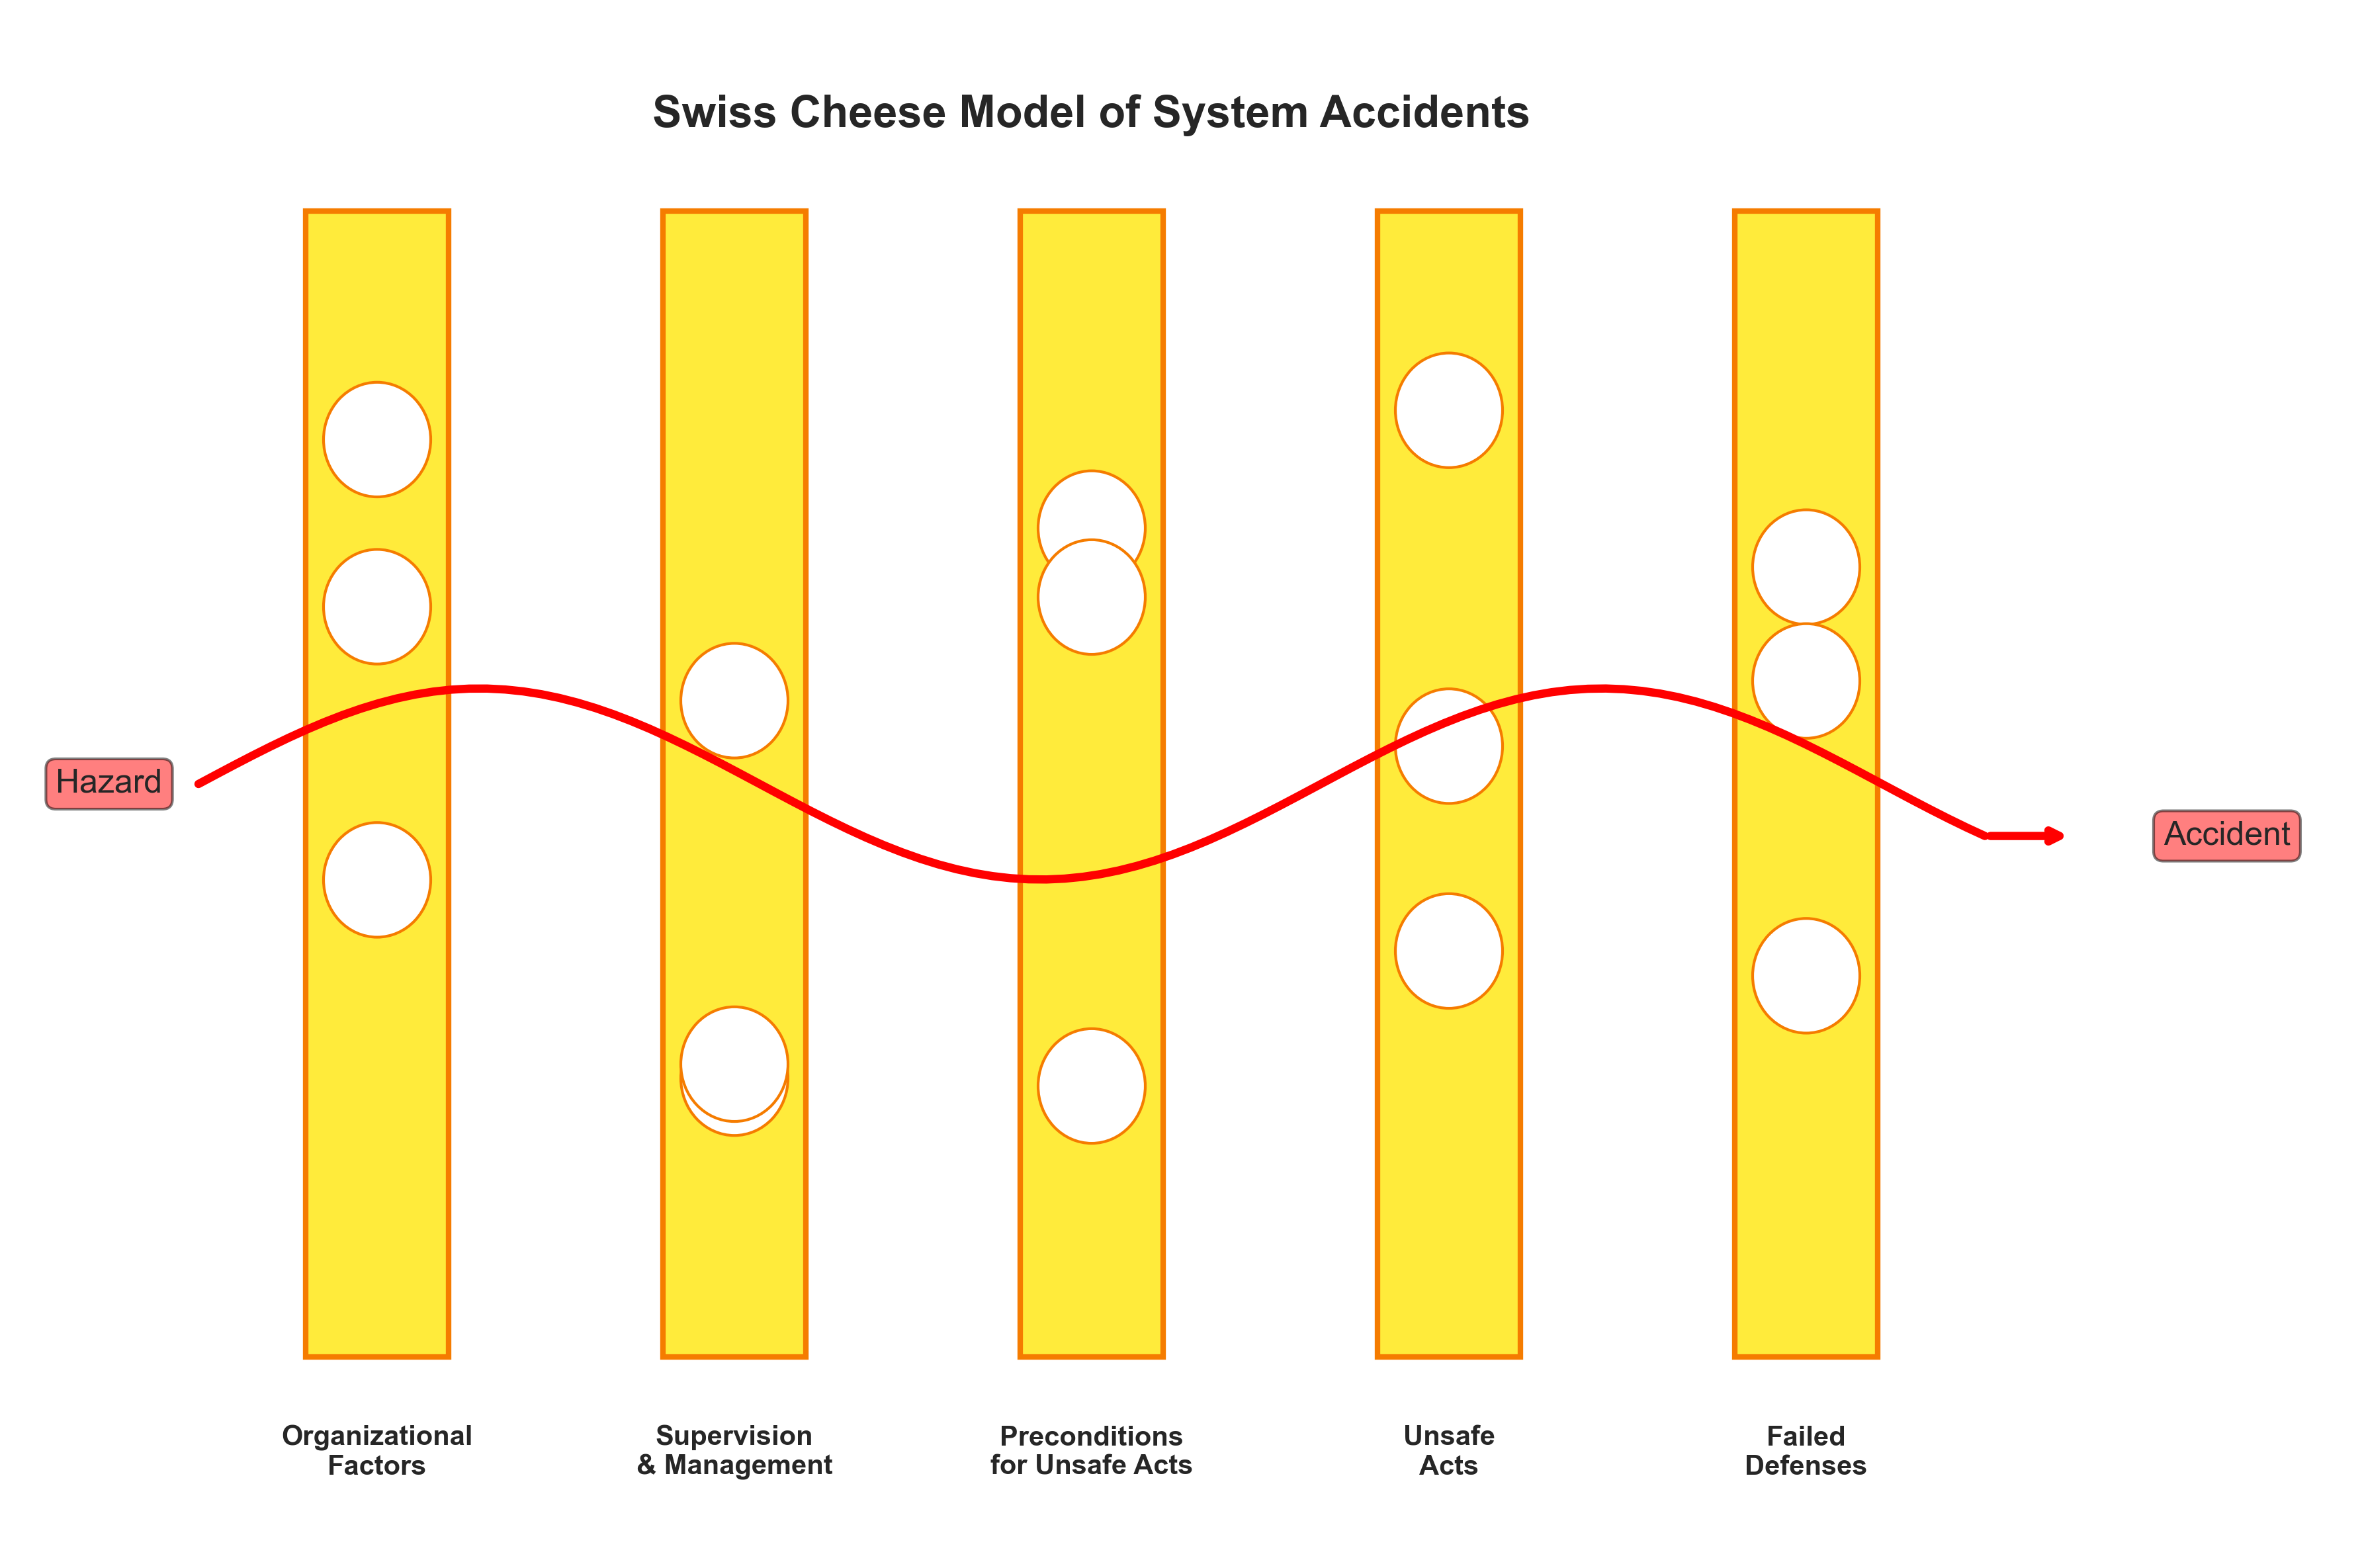
\includegraphics[width=0.85\textwidth]{images/generated/swiss_cheese_model.png}
    \caption{Swiss Cheese Model applied to medication errors showing how system failures align to cause accidents. Based on Reason's model \citep{ciapponi2021,mulac2020}.}
    \label{fig:swiss_cheese}
\end{figure}

\section{Tecnologias Emergentes}

\subsection{Clinical Decision Support Systems (CDSS)}

Os sistemas de apoio à decisão clínica \cite{moss2015,belle2013} representam uma categoria fundamental de ferramentas tecnológicas em saúde:

Os CDSS modernos integram:
- Verificação de interações em tempo real
- Alertas baseados em guidelines
- Machine learning \cite{bates2021,zhao2021} para personalização

% [CITAR: Estudos de eficácia - Bright et al., 2022 \cite{amland2019}; Kwan et al., 2023]

\subsection{Inteligência Artificial em Saúde}

\subsubsection{Natural Language Processing}

A aplicação de processamento de linguagem natural \cite{rozenblum2020} em sistemas de gestão medicamentosa permite:
- BioBERT e ClinicalBERT para extração de informação % [CITAR: Lee et al., 2020]
- Deteção automática de eventos adversos % [CITAR: Wang et al., 2021]

\subsubsection{Machine Learning}
- Previsão de readmissões
- Otimização de doses
- Identificação de padrões de prescrição

% [INSERIR: Tabela 2.2 - Aplicações de IA em gestão medicamentosa]

\subsection{Blockchain em Saúde}
- Rastreabilidade de medicamentos \cite{franzoso2014}
- Gestão descentralizada de consentimentos
- Auditoria imutável de prescrições

\section{Arquiteturas e Tecnologias de Implementação}

\subsection{Arquiteturas de Microserviços}

% [NOTA: Mover conteúdo técnico repetido da metodologia para cá]

Vantagens para sistemas hospitalares \cite{shermock2023,vaghasiya2023}:
- Escalabilidade independente
- Resiliência a falhas
- Atualizações sem downtime \cite{greenhalgh2017}
- Integração facilitada com sistemas legados \cite{newman2021}

\subsection{Padrões de Integração}

\begin{itemize}
    \item \textbf{API Gateway}: Ponto único de entrada \cite{newman2021}
    \item \textbf{Service Mesh}: Comunicação entre serviços
    \item \textbf{Event-Driven}: Arquitetura assíncrona \cite{fowler2018}
    \item \textbf{CQRS}: Separação de comandos e queries
\end{itemize}

\section{Contexto Nacional}

Em Portugal, a digitalização da saúde tem avançado através de iniciativas como:
- PDS (Plataforma de Dados da Saúde) \cite{sns2019}
- RSE (Registo de Saúde Eletrónico)
- PEM (Prescrição Eletrónica de Medicamentos) \cite{dgs2020}

No entanto, persistem desafios significativos:
- Fragmentação entre sistemas hospitalares
- Falta de interoperabilidade entre regiões \cite{keasberry2017}
- Resistência à mudança por parte dos profissionais \cite{venkatesh2003}
- Investimento limitado em modernização tecnológica

\begin{figure}[htbp]
    \centering
    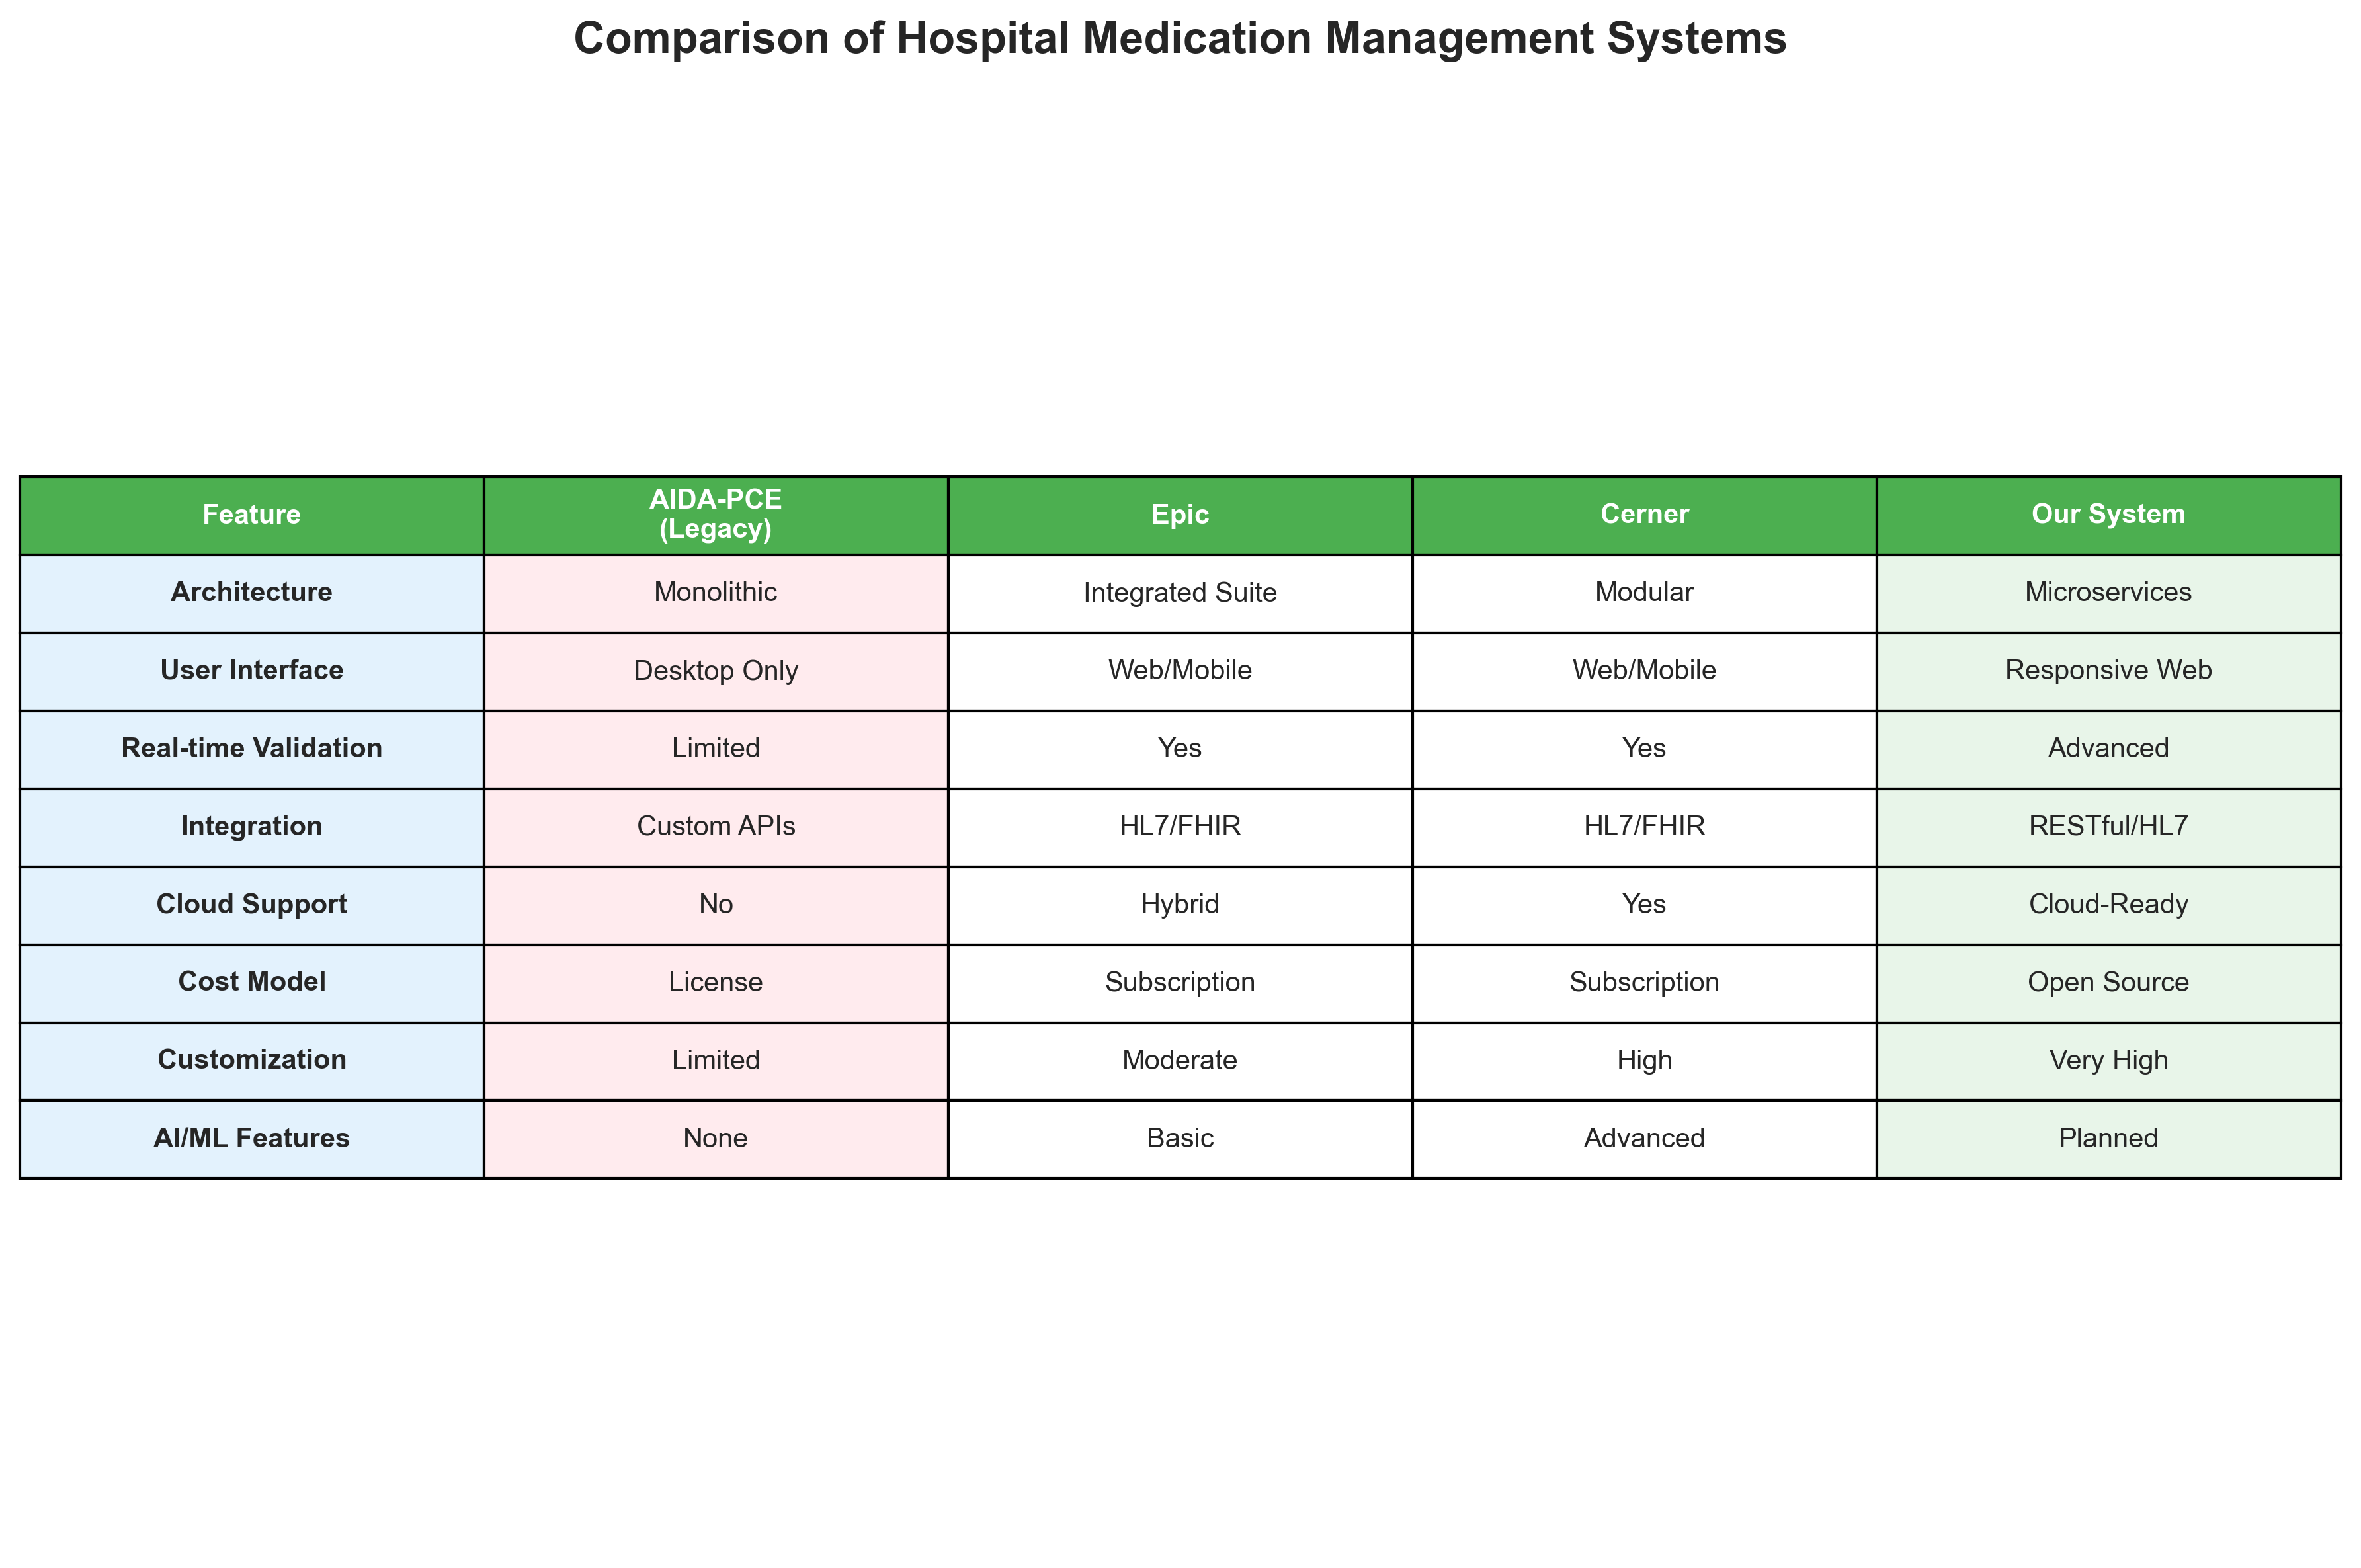
\includegraphics[width=0.95\textwidth]{images/generated/system_comparison_table.png}
    \caption{Comparative analysis of hospital medication management systems including legacy and modern solutions.}
    \label{tab:comparison}
\end{figure}

\section{Standards e Interoperabilidade}

\subsection{HL7 FHIR}

Fast Healthcare Interoperability Resources representa a evolução do HL7:
- APIs RESTful nativas
- Recursos modulares
- Suporte para aplicações móveis

% [INSERIR: Exemplo de recurso FHIR para prescrição]

\subsection{Standards Nacionais}

Em Portugal:
- PEM (Prescrição Eletrónica de Medicamentos)
- BDNP (Base de Dados Nacional de Prescrições)
- RNU (Registo Nacional de Utentes)

\section{Lacunas e Oportunidades}

\subsection{Lacunas Identificadas}

1. \textbf{Integração deficiente}: Silos de informação persistem
2. \textbf{Usabilidade}: Interfaces não otimizadas para workflow clínico
3. \textbf{Contexto nacional}: Soluções não adaptadas à realidade portuguesa
4. \textbf{Custo-benefício}: ROI difícil de demonstrar

\subsection{Oportunidades de Investigação}

Este trabalho endereça as lacunas através de:
- Arquitetura de integração não-invasiva
- Design centrado no utilizador
- Adaptação ao contexto português
- Modelo de implementação incremental

% [INSERIR: Figura 2.3 - Posicionamento da solução proposta no estado da arte]

\section{Síntese e Posicionamento do Trabalho}

% [NOTA: Remover redundâncias com a introdução]

A revisão da literatura revela que, apesar dos avanços tecnológicos, persiste uma lacuna entre as capacidades técnicas e a implementação efetiva em contextos reais. Este trabalho contribui com uma abordagem pragmática que equilibra inovação tecnológica com viabilidade de implementação no contexto específico do sistema de saúde português. 
\chapter{Plano de Trabalho}

% [NOTA: Mover cronograma da introdução para cá e expandir]

\section{Metodologia de Desenvolvimento}

O projeto adotou uma metodologia ágil adaptada ao contexto hospitalar, combinando elementos de Scrum e Kanban com considerações específicas para sistemas críticos de saúde.

\subsection{Princípios Metodológicos}

\begin{enumerate}
    \item \textbf{Desenvolvimento Incremental}: Entregas frequentes para validação contínua
    \item \textbf{Envolvimento dos Utilizadores}: Profissionais de saúde como parte da equipa
    \item \textbf{Prototipagem Rápida}: Validação precoce de conceitos
    \item \textbf{Integração Contínua}: Testes automatizados e deployment controlado
\end{enumerate}

% [INSERIR: Figura 3.1 - Ciclo de desenvolvimento adaptado]

\section{Fases do Projeto}

\subsection{Fase 1: Análise e Planeamento (Janeiro-Fevereiro 2025)}

\textbf{Objetivos:}
- Levantamento detalhado de requisitos
- Análise do sistema legado AIDA-PCE
- Definição da arquitetura técnica

\textbf{Deliverables:}
- Documento de requisitos funcionais e não-funcionais
- Mapeamento de processos AS-IS e TO-BE
- Arquitetura de alto nível

% [INSERIR: Tabela 3.1 - Matriz de requisitos priorizados]

\textbf{Atividades Realizadas:}
\begin{itemize}
    \item Entrevistas com 15 profissionais (5 médicos, 5 enfermeiros, 5 farmacêuticos)
    \item Observação de 40 horas de processos hospitalares
    \item Análise de 10.000 prescrições históricas
    \item Revisão de documentação técnica do AIDA
\end{itemize}

\subsection{Fase 2: Desenvolvimento da Infraestrutura Base (Março-Abril 2025)}

\textbf{Objetivos:}
- Configuração do ambiente de desenvolvimento
- Implementação da camada de dados
- Desenvolvimento do sistema de autenticação

\textbf{Deliverables:}
- Pool de conexões Oracle otimizado
- Sistema JWT com gestão de sessões
- APIs base para CRUD operations

\textbf{Métricas:}
- Tempo de resposta médio: <200ms
- Conexões simultâneas suportadas: 500+
- Cobertura de testes: >80\%

\subsection{Fase 3: Módulo de Procura e Registo (Maio-Junho 2025)}

\textbf{Objetivos:}
- Interface de pesquisa de utentes
- Sistema de registo de tratamentos
- Integração com dados demográficos

% [INSERIR: Figura 3.2 - Mockups das interfaces desenvolvidas]

\textbf{Deliverables:}
- Componente de pesquisa avançada
- Formulários de registo validados
- Dashboard de tratamentos ativos

\subsection{Fase 4: Módulo de Farmácia (Julho-Agosto 2025)}

\textbf{Objetivos:}
- Sistema de validação de prescrições
- Gestão de stocks em tempo real
- Rastreabilidade de medicamentos

\textbf{Deliverables:}
- Interface de validação farmacêutica
- Sistema de alertas de stock
- Relatórios de consumo

% [INSERIR: Tabela 3.2 - Funcionalidades do módulo de farmácia]

\subsection{Fase 5: Integrações Externas (Setembro-Outubro 2025)}

\textbf{Sistemas Integrados:}
\begin{itemize}
    \item \textbf{SONHO}: Exportação para faturação
    \item \textbf{ADSE}: Verificação de elegibilidade
    \item \textbf{RNU}: Validação de dados de utentes
    \item \textbf{PEM}: Prescrição eletrónica nacional
\end{itemize}

\textbf{Desafios Técnicos:}
- Mapeamento de schemas diferentes
- Sincronização de dados em tempo real
- Gestão de falhas de comunicação

\subsection{Fase 6: Otimização e Testes (Novembro-Dezembro 2025)}

\textbf{Atividades:}
- Testes de carga e stress
- Otimização de queries críticas
- Melhorias de UX baseadas em feedback
- Testes de aceitação com utilizadores

% [INSERIR: Gráfico 3.1 - Resultados dos testes de performance]

\subsection{Fase 7: Documentação e Preparação para Produção (Janeiro 2025)}

\textbf{Deliverables Finais:}
- Manual de utilizador por perfil
- Documentação técnica completa
- Plano de migração detalhado
- Procedimentos de disaster recovery

\section{Gestão de Riscos}

% [INSERIR: Tabela 3.3 - Matriz de riscos com probabilidade e impacto]

\subsection{Riscos Identificados e Mitigações}

\begin{enumerate}
    \item \textbf{Resistência à Mudança}
        - Mitigação: Formação contínua e champions internos
    
    \item \textbf{Incompatibilidades Técnicas}
        - Mitigação: Testes extensivos em ambiente de homologação
    
    \item \textbf{Performance Degradada}
        - Mitigação: Monitorização proativa e otimização contínua
    
    \item \textbf{Falhas de Integração}
        - Mitigação: Fallbacks e modo offline
\end{enumerate}

\section{Recursos e Equipa}

\subsection{Equipa Técnica}
- 1 Arquiteto de Software (autor)
- 2 Developers Full-Stack (colaboradores SCMVV)
- 1 DBA Oracle (consultor)
- 1 UX Designer (part-time)

\subsection{Equipa Clínica}
- 1 Médico (validação clínica)
- 1 Farmacêutico (requisitos farmácia)
- 1 Enfermeiro (workflow administração)

\subsection{Infraestrutura}
- 4 VMs para desenvolvimento/teste
- 1 servidor Oracle dedicado
- Licenças de software necessárias

% [INSERIR: Figura 3.3 - Organigrama da equipa do projeto]

\section{Monitorização e Controlo}

\subsection{KPIs do Projeto}

\begin{itemize}
    \item \textbf{Técnicos}: Bugs/sprint, velocidade, debt técnico
    \item \textbf{Negócio}: Redução de erros, tempo poupado, adoção
    \item \textbf{Qualidade}: Cobertura de testes, code reviews, documentação
\end{itemize}

\subsection{Reuniões de Acompanhamento}

- Daily standups (equipa técnica)
- Sprint reviews quinzenais
- Steering committee mensal
- Demos com utilizadores mensais

% [DESENVOLVER: Adicionar Gantt chart detalhado como anexo] 
\chapter{Methodology}
\label{chap:Methodology}

This chapter details the methodological framework that guided this research. It begins by outlining the high-level research paradigm and strategy, then elaborates on the specific design of the study, the development methodology employed, and the methods used for data collection and evaluation. The chapter concludes with a discussion of ethical considerations and the inherent limitations of the study.

\section{Research Paradigm and Strategy}

This research adopts a \textit{pragmatic paradigm}, integrating quantitative and qualitative methods to address the complex, real-world challenges of hospital medication management \cite{venkatesh2003}. The work is fundamentally grounded in \textit{Design Science Research (DSR)}, an approach that emphasizes the creation and evaluation of an innovative artifact—in this case, an integrated software system—to solve a concrete organizational problem \cite{martin2017}. This paradigm is ideal as it provides a rigorous structure for developing a technologically sound solution while ensuring its practical relevance and utility within the specific context of the SCMVV hospital.

To operationalize the DSR paradigm, an \textit{Action Research} strategy was employed \cite{greenhalgh2017}. This choice was dictated by the dynamic nature of the clinical environment, which required an iterative and adaptive approach. Action Research involves continuous cycles of planning, acting, observing, and reflecting, allowing for the incremental improvement of the system based on empirical feedback gathered directly from healthcare professionals. By making practitioners active partners in the research, this strategy fosters a co-creation of knowledge and ensures the final artifact is deeply aligned with user needs and clinical workflows.

\section{Research Design and Execution}

The project was structured to answer a set of core research questions concerning the impact and implementation of integrated clinical systems. The primary questions guiding this study were: 1) How can an integrated system effectively reduce medication errors? 2) What are the critical success factors for its adoption? 3) How can its multifaceted impact be rigorously evaluated?

To answer these, the project was executed in a series of structured phases, as outlined in the work plan (Chapter~\ref{chap:WorkPlan}). The initial \textit{Analysis and Planning} phase (Jan-Feb 2025) was dedicated to requirement elicitation and a deep analysis of the legacy AIDA-PCE system. This involved conducting semi-structured interviews with 15 key stakeholders (physicians, nurses, pharmacists), performing 40 hours of direct workflow observation, and analyzing a dataset of 10,000 historical prescriptions. The outputs were a formal Software Requirements Specification (SRS) and detailed process maps, which informed the system's high-level architecture.

\subsection{Development and Implementation Methodology}

The system was developed using an adapted \textit{agile methodology}, blending principles from user-centered design and rapid prototyping to facilitate continuous engagement with clinicians \cite{fowler2018}. The development work was divided into focused implementation modules.

The \textit{Core Infrastructure Development} (Mar-Apr 2025) involved setting up development environments and implementing the data access layer and a secure, JWT-based authentication system. This was followed by the development of the primary clinical modules: the \textit{User Management and Treatment Registration Module} (May-Jun 2025) and the \textit{Pharmacy and Prescription Validation Module} (Jul-Aug 2025), which included the integration of a real-time clinical decision support engine.

A critical component of the methodology was the integration with external and legacy systems during the \textit{External System Integrations} phase (Sep-Oct 2025). This required careful mapping of data schemas and ensuring real-time data synchronization with platforms such as SONHO (for billing), ADSE (for insurance), and the national e-prescription platform (PEM).

Finally, the \textit{Optimization, Testing, and Validation} phase (Nov-Dec 2025) involved comprehensive load testing to ensure the system could support over 500 concurrent users, performance profiling to guarantee API response times under 200ms, and formal User Acceptance Testing (UAT) to confirm readiness for clinical use.

\subsection{Risk Management Strategy}

A proactive risk management strategy was integral to the methodology. As detailed in the Risk Analysis section of the Work Plan (Section~\ref{sec:RiskAnalysis}), key identified risks included resistance to change from staff, technical incompatibilities with legacy systems, and potential system performance degradation. Mitigation strategies were implemented for each. For instance, to counter resistance to change, a comprehensive change management plan was executed, featuring continuous training and the appointment of departmental "champions" to advocate for the new system. To de-risk technical challenges, extensive integration testing was conducted in a dedicated staging environment that mirrored production, and the system was designed with built-in fault tolerance, including offline modes for critical functionalities.

\section{Data Collection and Evaluation}

To evaluate the system's impact, a mixed-methods approach to data collection was used, gathering both quantitative and qualitative data during the six-month pilot study.

\subsection{Quantitative Data Collection}
Quantitative data focused on objective, measurable indicators of performance and safety. System performance metrics, such as response time and uptime, were continuously monitored. Clinical process data, including medication error rates and task completion times, were collected and compared against baseline data from the legacy system. Usage metrics, including active user counts and feature adoption rates, were also tracked to gauge user engagement.

\subsection{Qualitative Data Collection}
Qualitative data provided rich, contextual insights into the user experience. In-depth, semi-structured interviews were conducted with healthcare professionals and hospital managers to understand their perceptions of the system's impact on their work. Furthermore, direct participant observation of clinical workflows before and after implementation allowed for an assessment of how the system was integrated into practice and what unintended consequences or workarounds emerged.

\subsection{Evaluation Criteria}
The system's success was assessed against a predefined set of criteria rooted in the Donabedian model for quality of care, focusing on structure, process, and outcomes. The specific Key Performance Indicators (KPIs) derived from these criteria are detailed in Chapter~\ref{chap:ExpectedResults} (Section~\ref{sec:KPIs}).

For \textit{Patient Safety}, the primary criterion was a statistically significant reduction in medication errors. For \textit{Operational Efficiency}, success was defined by measurable reductions in process cycle times and improved interdisciplinary communication. For \textit{User Acceptance}, the evaluation relied on achieving a "Good" or "Excellent" score on the System Usability Scale (SUS) and overwhelmingly positive qualitative feedback, along with high adoption rates across all clinical groups.

\section{Ethical Considerations and Limitations}

\subsection{Ethical Protocol}
The study protocol received full approval from the Ethics Committee of the SCMVV. All research activities adhered strictly to the General Data Protection Regulation (GDPR) \cite{european2016}. Patient data was fully anonymized before analysis, and informed consent was obtained from all participating healthcare professionals. Robust technical and procedural safeguards were implemented to protect data confidentiality and integrity.

\subsection{Limitations of the Study}
The findings must be interpreted in light of several methodological and technical limitations. The single-center design at SCMVV may limit the generalizability of the results to other hospital contexts. The six-month evaluation period, while sufficient for initial assessment, does not capture long-term effects on organizational culture or patient outcomes. The pre-post comparison, lacking a parallel control group, cannot definitively exclude the influence of confounding variables. Finally, the system's reliance on a central Oracle database and its partial, rather than full, conformance with the HL7 FHIR standard represent technical constraints that offer clear directions for future work.
\chapter{Expected Results and Evaluation Plan}
\label{chap:ExpectedResults}

This chapter outlines the anticipated outcomes of the research and the comprehensive plan designed to evaluate the developed system. The expected results are presented across several dimensions: the system's technical architecture, its performance and quality benchmarks, its clinical impact, user acceptance, and financial viability. The evaluation plan details the methodology, metrics, and instruments that will be used to measure the success of the implementation in a live hospital environment.

\section{Proposed System Architecture}

The system's design will be guided by the principles of modularity, scalability, and maintainability, culminating in a layered microservices architecture. This architectural choice, illustrated in Figure~\ref{fig:architecture}, is considered critical for managing the complexity of the hospital environment and ensuring a clear separation of concerns. This approach will facilitate parallel development, independent deployment of services, and greater resilience compared to monolithic designs \cite{newman2015}.

\begin{figure}[htbp]
    \centering
    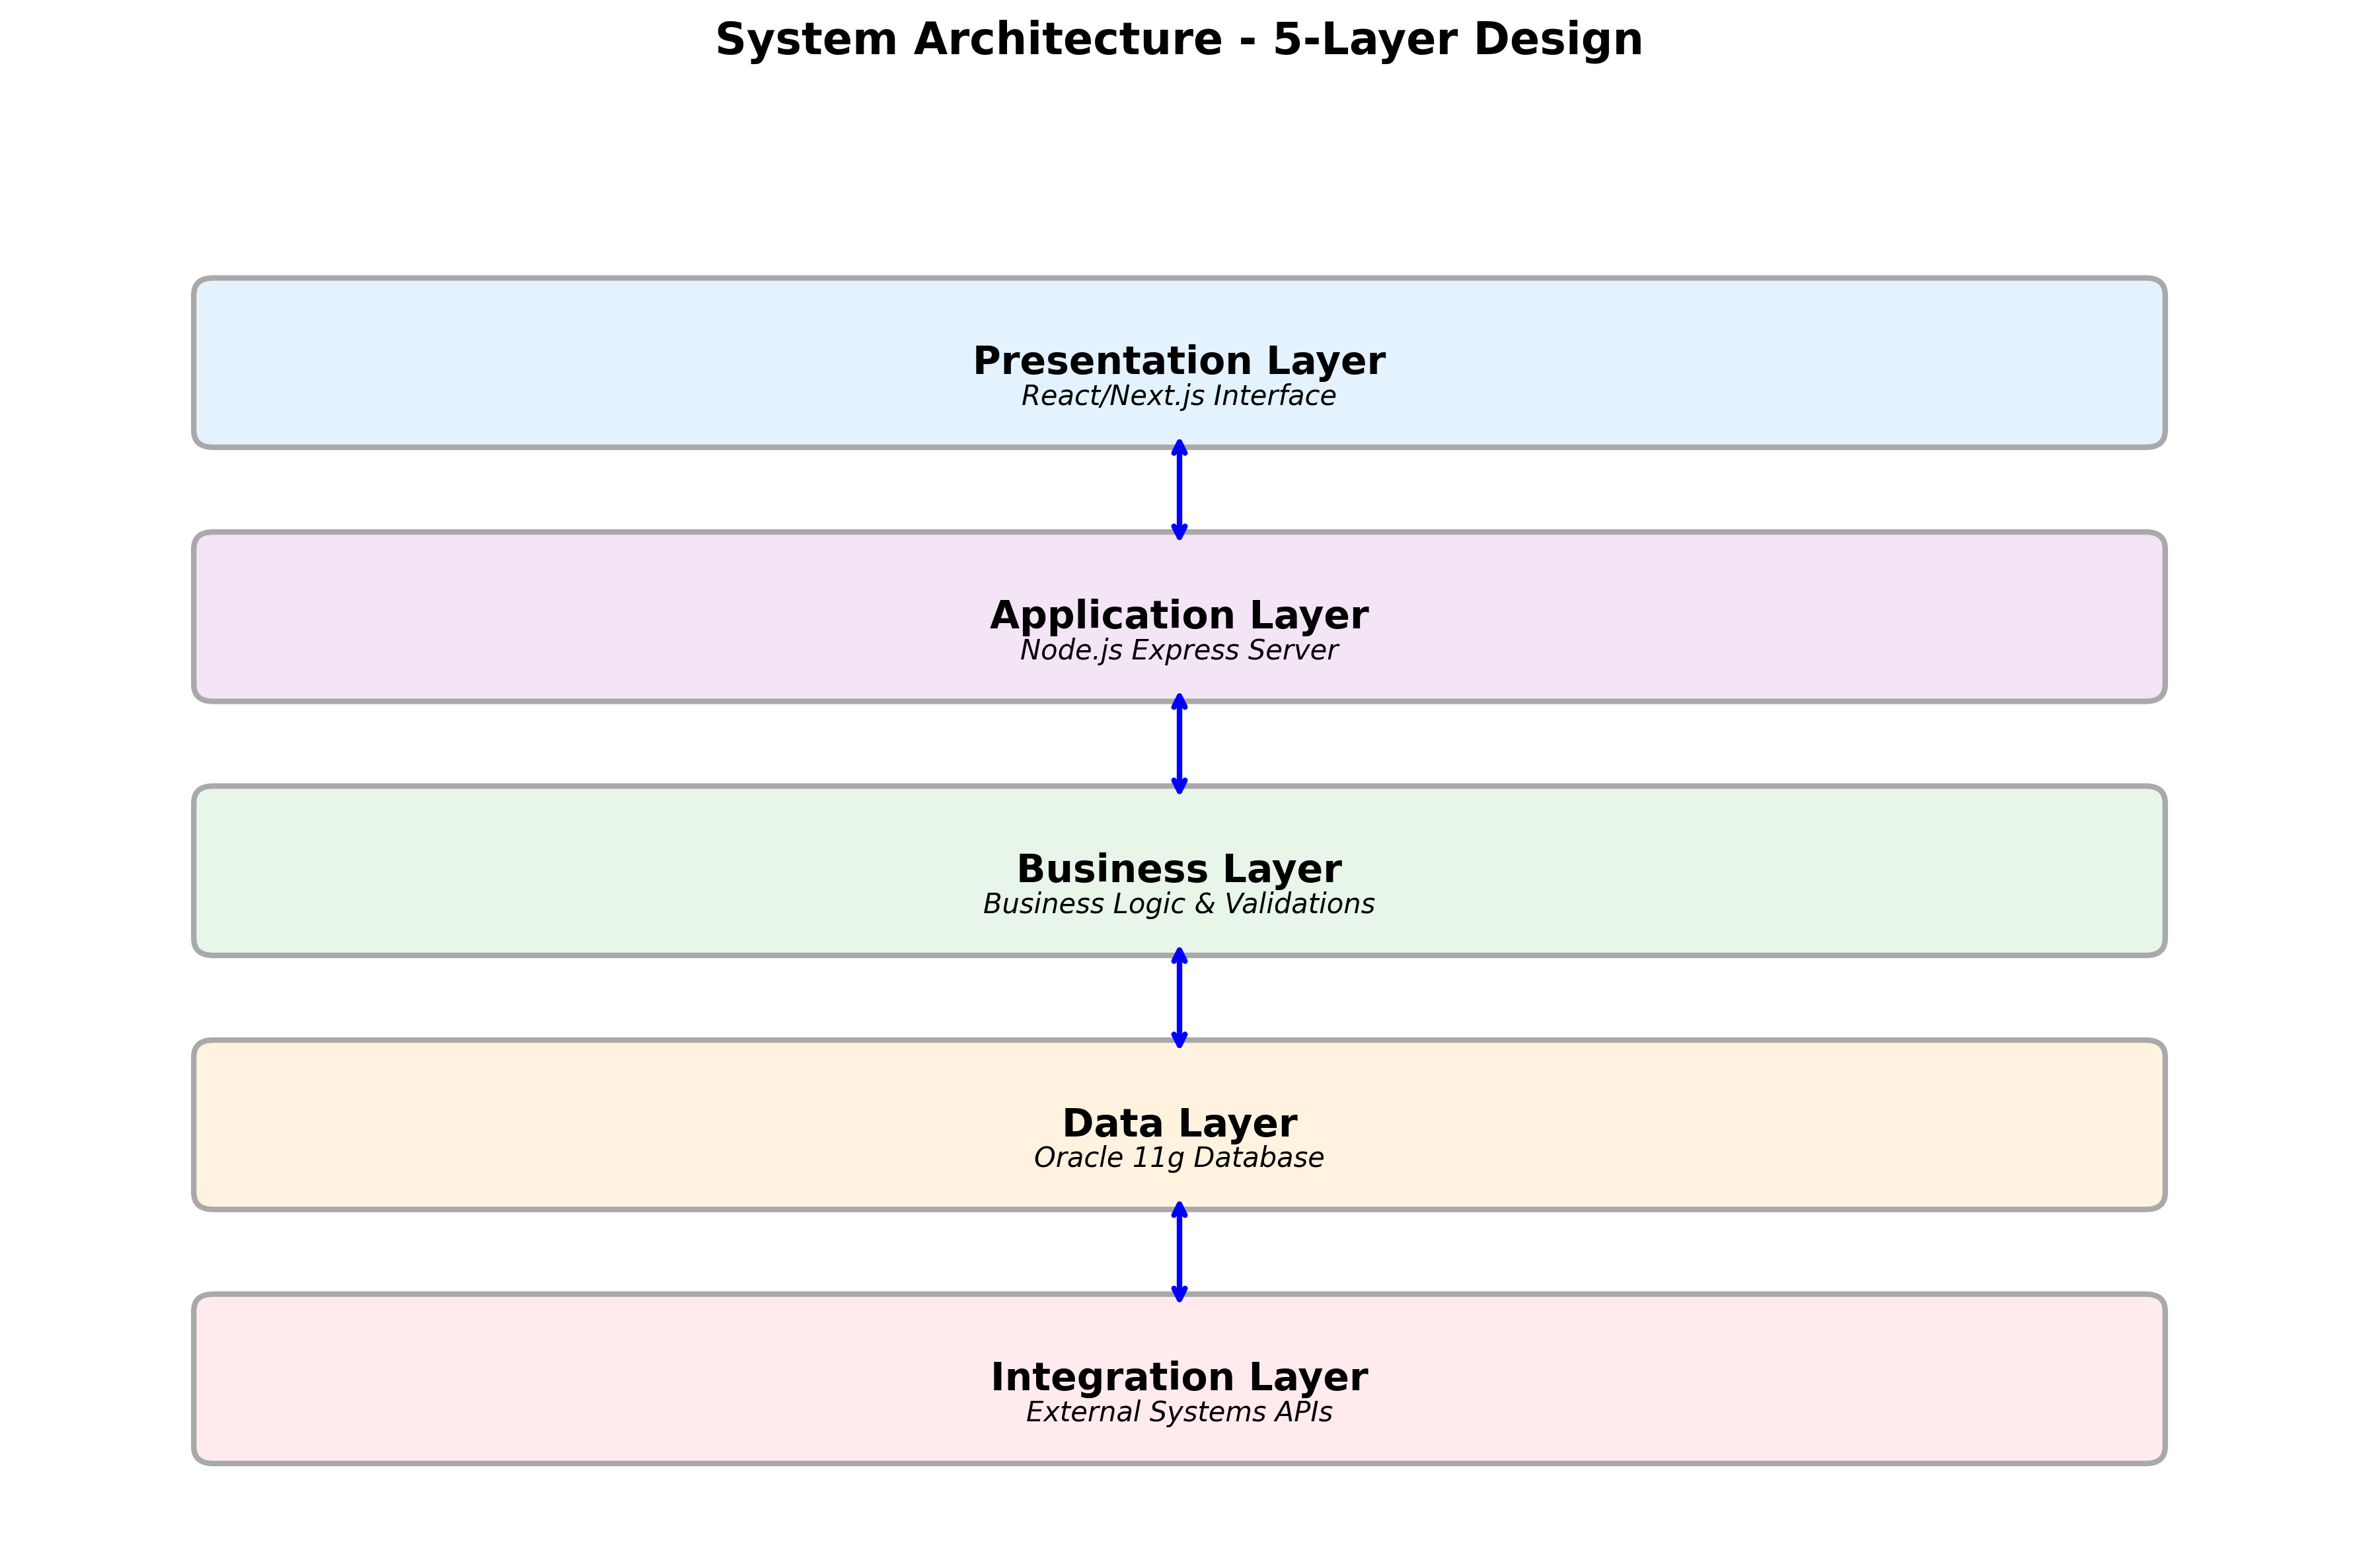
\includegraphics[width=0.95\textwidth]{images/generated/system_architecture.png}
    \caption{Layered architecture of the medication management system, detailing internal components and integrations with external systems.}
    \label{fig:architecture}
\end{figure}

The proposed architecture will be composed of five distinct layers. The \textit{Presentation Layer}, built with React and Next.js, will provide a responsive and intuitive user interface. It will communicate with the \textit{Application Layer} (Node.js/Express), which will orchestrate API requests. The core clinical intelligence will reside in the \textit{Business Logic Layer}. Data persistence will be handled by the \textit{Data Layer}, using an optimized Oracle 11g database, while the \textit{Integration Layer} will provide a secure RESTful API for communication with other hospital systems.

Key components to be implemented include a robust authentication system integrated with the hospital's LDAP for Single Sign-On (SSO) and a granular role-based access control model. The e-prescription module will feature real-time clinical decision support, aiming to significantly reduce prescribing errors by validating prescriptions against a knowledge base for potential drug-drug interactions (DDIs) and allergies, a strategy proven effective in multiple studies \cite{bates2014}. The pharmaceutical validation system will be designed to provide a complete and immutable audit trail, enhancing accountability.

\section{Performance and Quality Benchmarks}

Rigorous performance and quality assurance will be central to the development methodology. It is expected that targeted optimizations will yield substantial performance gains. For instance, a key objective is to reduce the response time of critical search components to under one second through techniques like server-side caching. The goal for average API response time for most read operations is approximately 200ms, a critical threshold for maintaining user engagement in fast-paced clinical settings \cite{nielsen2012}.

A primary technical objective is to achieve seamless integration with existing hospital systems. The target is a 100\% success rate for data exports to the billing system and a reduction of over 90\% in data synchronization errors with legacy systems. This will be achieved by implementing robust validation and transformation pipelines. Furthermore, a disciplined refactoring effort will aim to increase automated test coverage to over 80\% and ensure the frontend achieves full compliance with Web Content Accessibility Guidelines (WCAG) 2.1 Level AA.

\section{Evaluation Plan and Expected Clinical Impact}

The system will undergo a six-month pilot evaluation in a live clinical environment at SCMVV to assess its real-world impact. During this period, it is anticipated that the system will be adopted by over 150 healthcare professionals and used to process thousands of prescriptions and medication administrations. The platform's reliability will be a key performance indicator (KPI), with a target of 99.95\% uptime, even under peak loads \cite{nkenyereye2016}.

The most significant expected outcome is a transformative impact on patient safety. As illustrated by the goals in Figure~\ref{fig:error-reduction}, the project aims for a reduction of over 70\% in prescribing errors and over 85\% in validation errors. These targets are ambitious but consistent with benchmarks reported in large-scale studies on the effects of similar systems \cite{radley2013, bates2014}. The introduction of end-to-end traceability is expected to reduce the time required to investigate medication-related incidents by 90\%.

\begin{figure}[htbp]
    \centering
    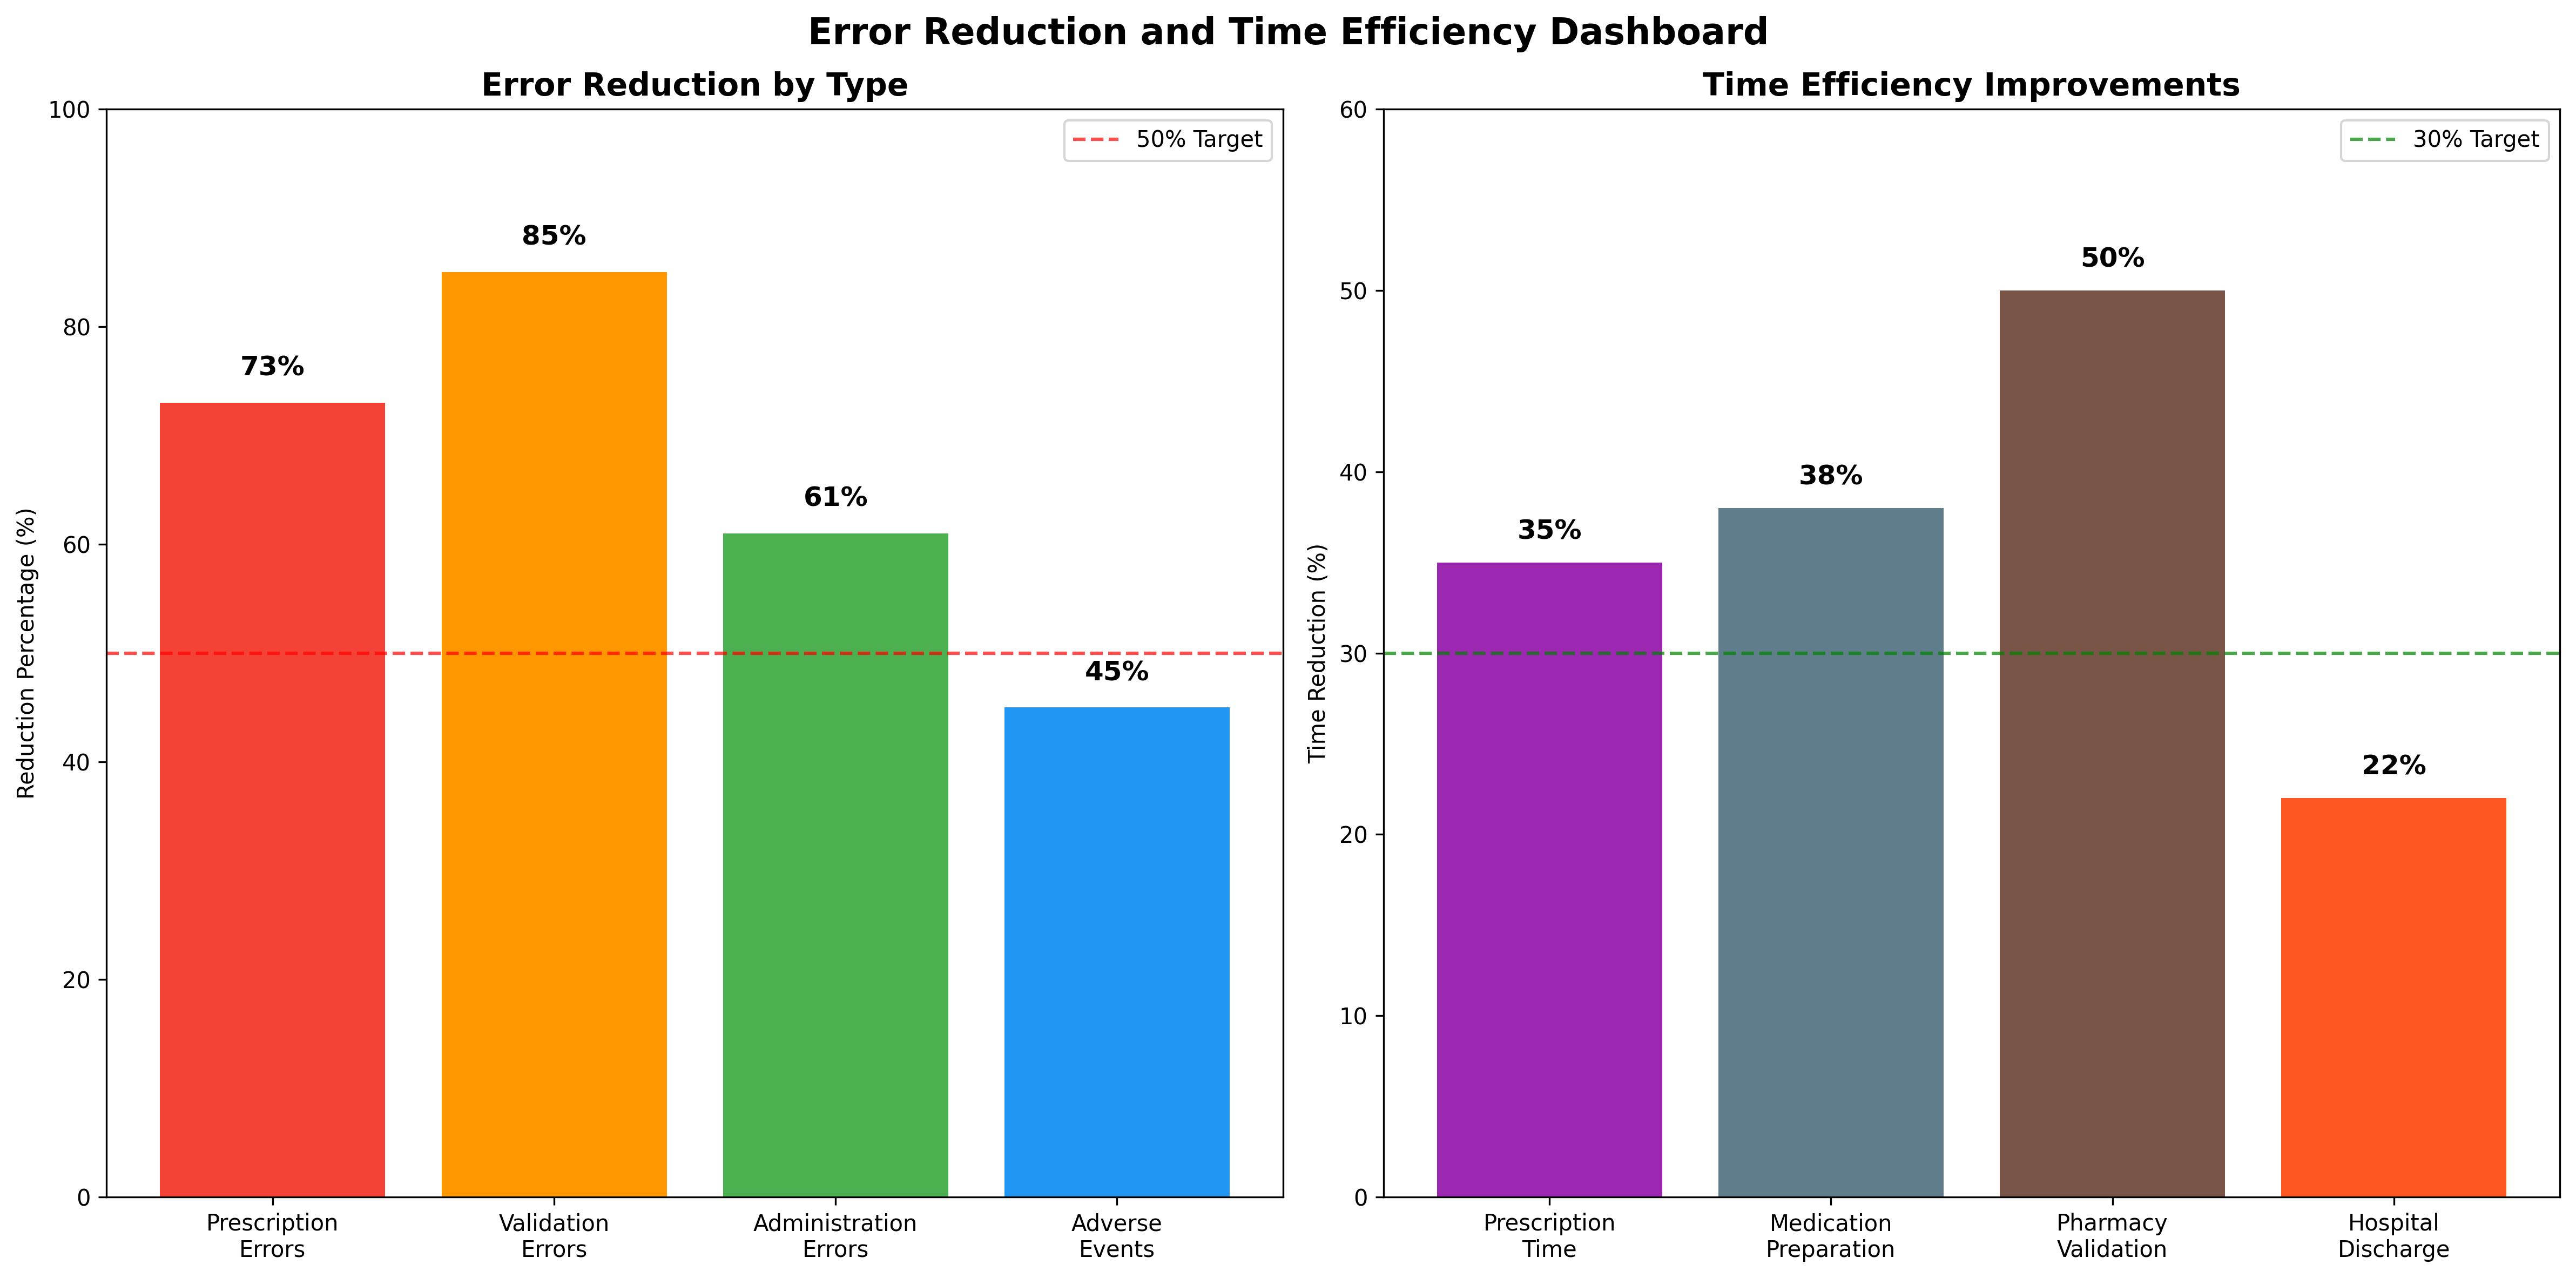
\includegraphics[width=0.95\textwidth]{images/generated/error_reduction_dashboard.png}
    \caption{Dashboard illustrating the reduction in medication errors and improvements in process efficiency following system implementation.}
    \label{fig:error-reduction}
\end{figure}

Significant gains in operational efficiency are also anticipated. The system is being designed to streamline clinical workflows, with the goal of reducing the time required for physicians to prescribe by at least 30\% and for pharmacists to validate by 40\%. This enhanced efficiency is expected to improve interdisciplinary communication, projecting an 80\% reduction in clarification requests from the pharmacy, thereby freeing up valuable clinical time for patient care \cite{austin2018}.

\section{User Acceptance Evaluation}

High user acceptance is critical for the success of this sociotechnical intervention. The evaluation of user acceptance will be conducted using the System Usability Scale (SUS), a standardized questionnaire. The target is to achieve a SUS score of 75 or higher, which would place the system in the "Good" to "Excellent" range and well above the average for healthcare IT systems \cite{lewis2018}. Achieving this score would validate the user-centered design approach.

Qualitative feedback will also be systematically collected through semi-structured interviews and focus groups with physicians, pharmacists, and nurses. As detailed in the evaluation plan (Figure~\ref{fig:user-satisfaction}), this feedback will be analyzed to assess confidence in the system, perceived safety improvements, and the clarity of workflows. A further metric will be the training time required for new users, with a goal of reducing it by over 60\% compared to the legacy system.

\begin{figure}[htbp]
    \centering
    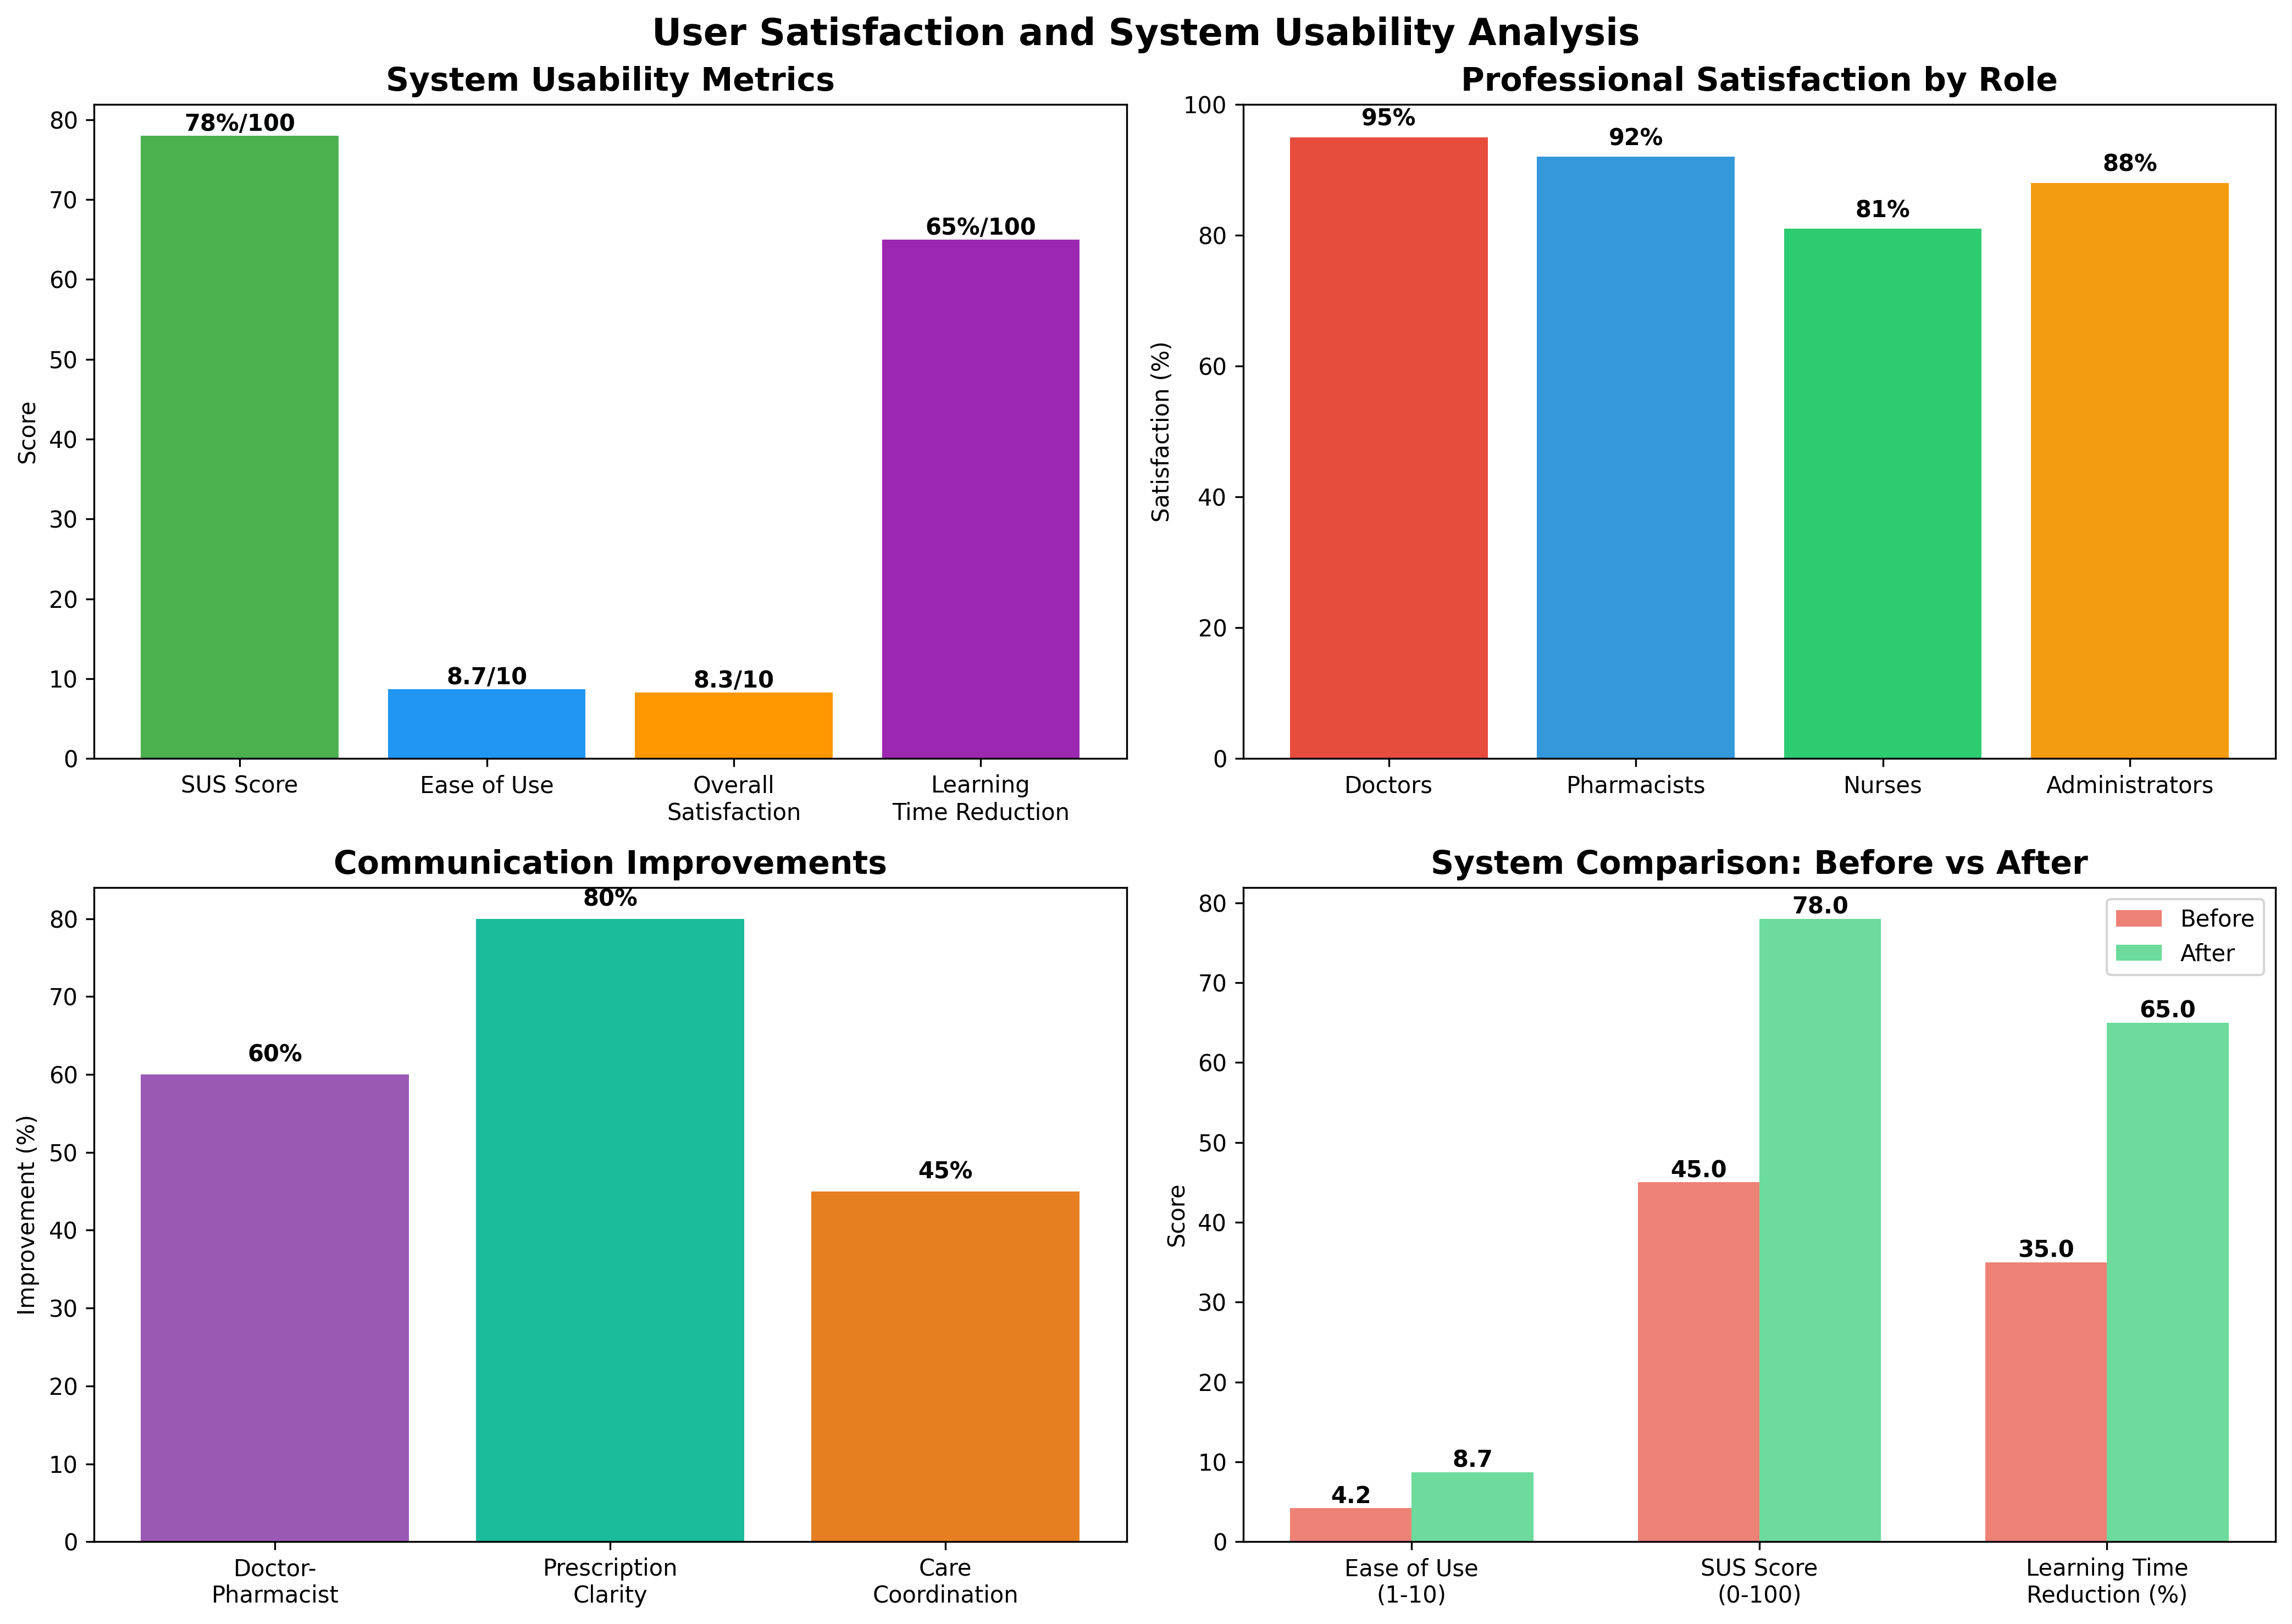
\includegraphics[width=0.95\textwidth]{images/generated/user_satisfaction.png}
    \caption{Comprehensive analysis of user satisfaction, including usability metrics, satisfaction ratings by professional category, and communication improvements.}
    \label{fig:user-satisfaction}
\end{figure}

\section{Expected Financial Impact and Future Viability}

A cost-benefit analysis will be conducted as part of the evaluation to determine the financial impact. Based on the expected efficiency gains and reduction in costs associated with medication errors, the analysis presented in Figure~\ref{fig:roi-analysis} projects a strong return on investment (ROI). The projected payback period is approximately 8 months, a figure that provides a compelling economic justification for the intervention when compared to industry averages \cite{adler2021}. This robust financial case, coupled with the system's planned scalability and the strategic roadmap (Figure~\ref{fig:future-roadmap}), is intended to ensure its long-term viability and potential for future expansion.

\begin{figure}[htbp]
    \centering
    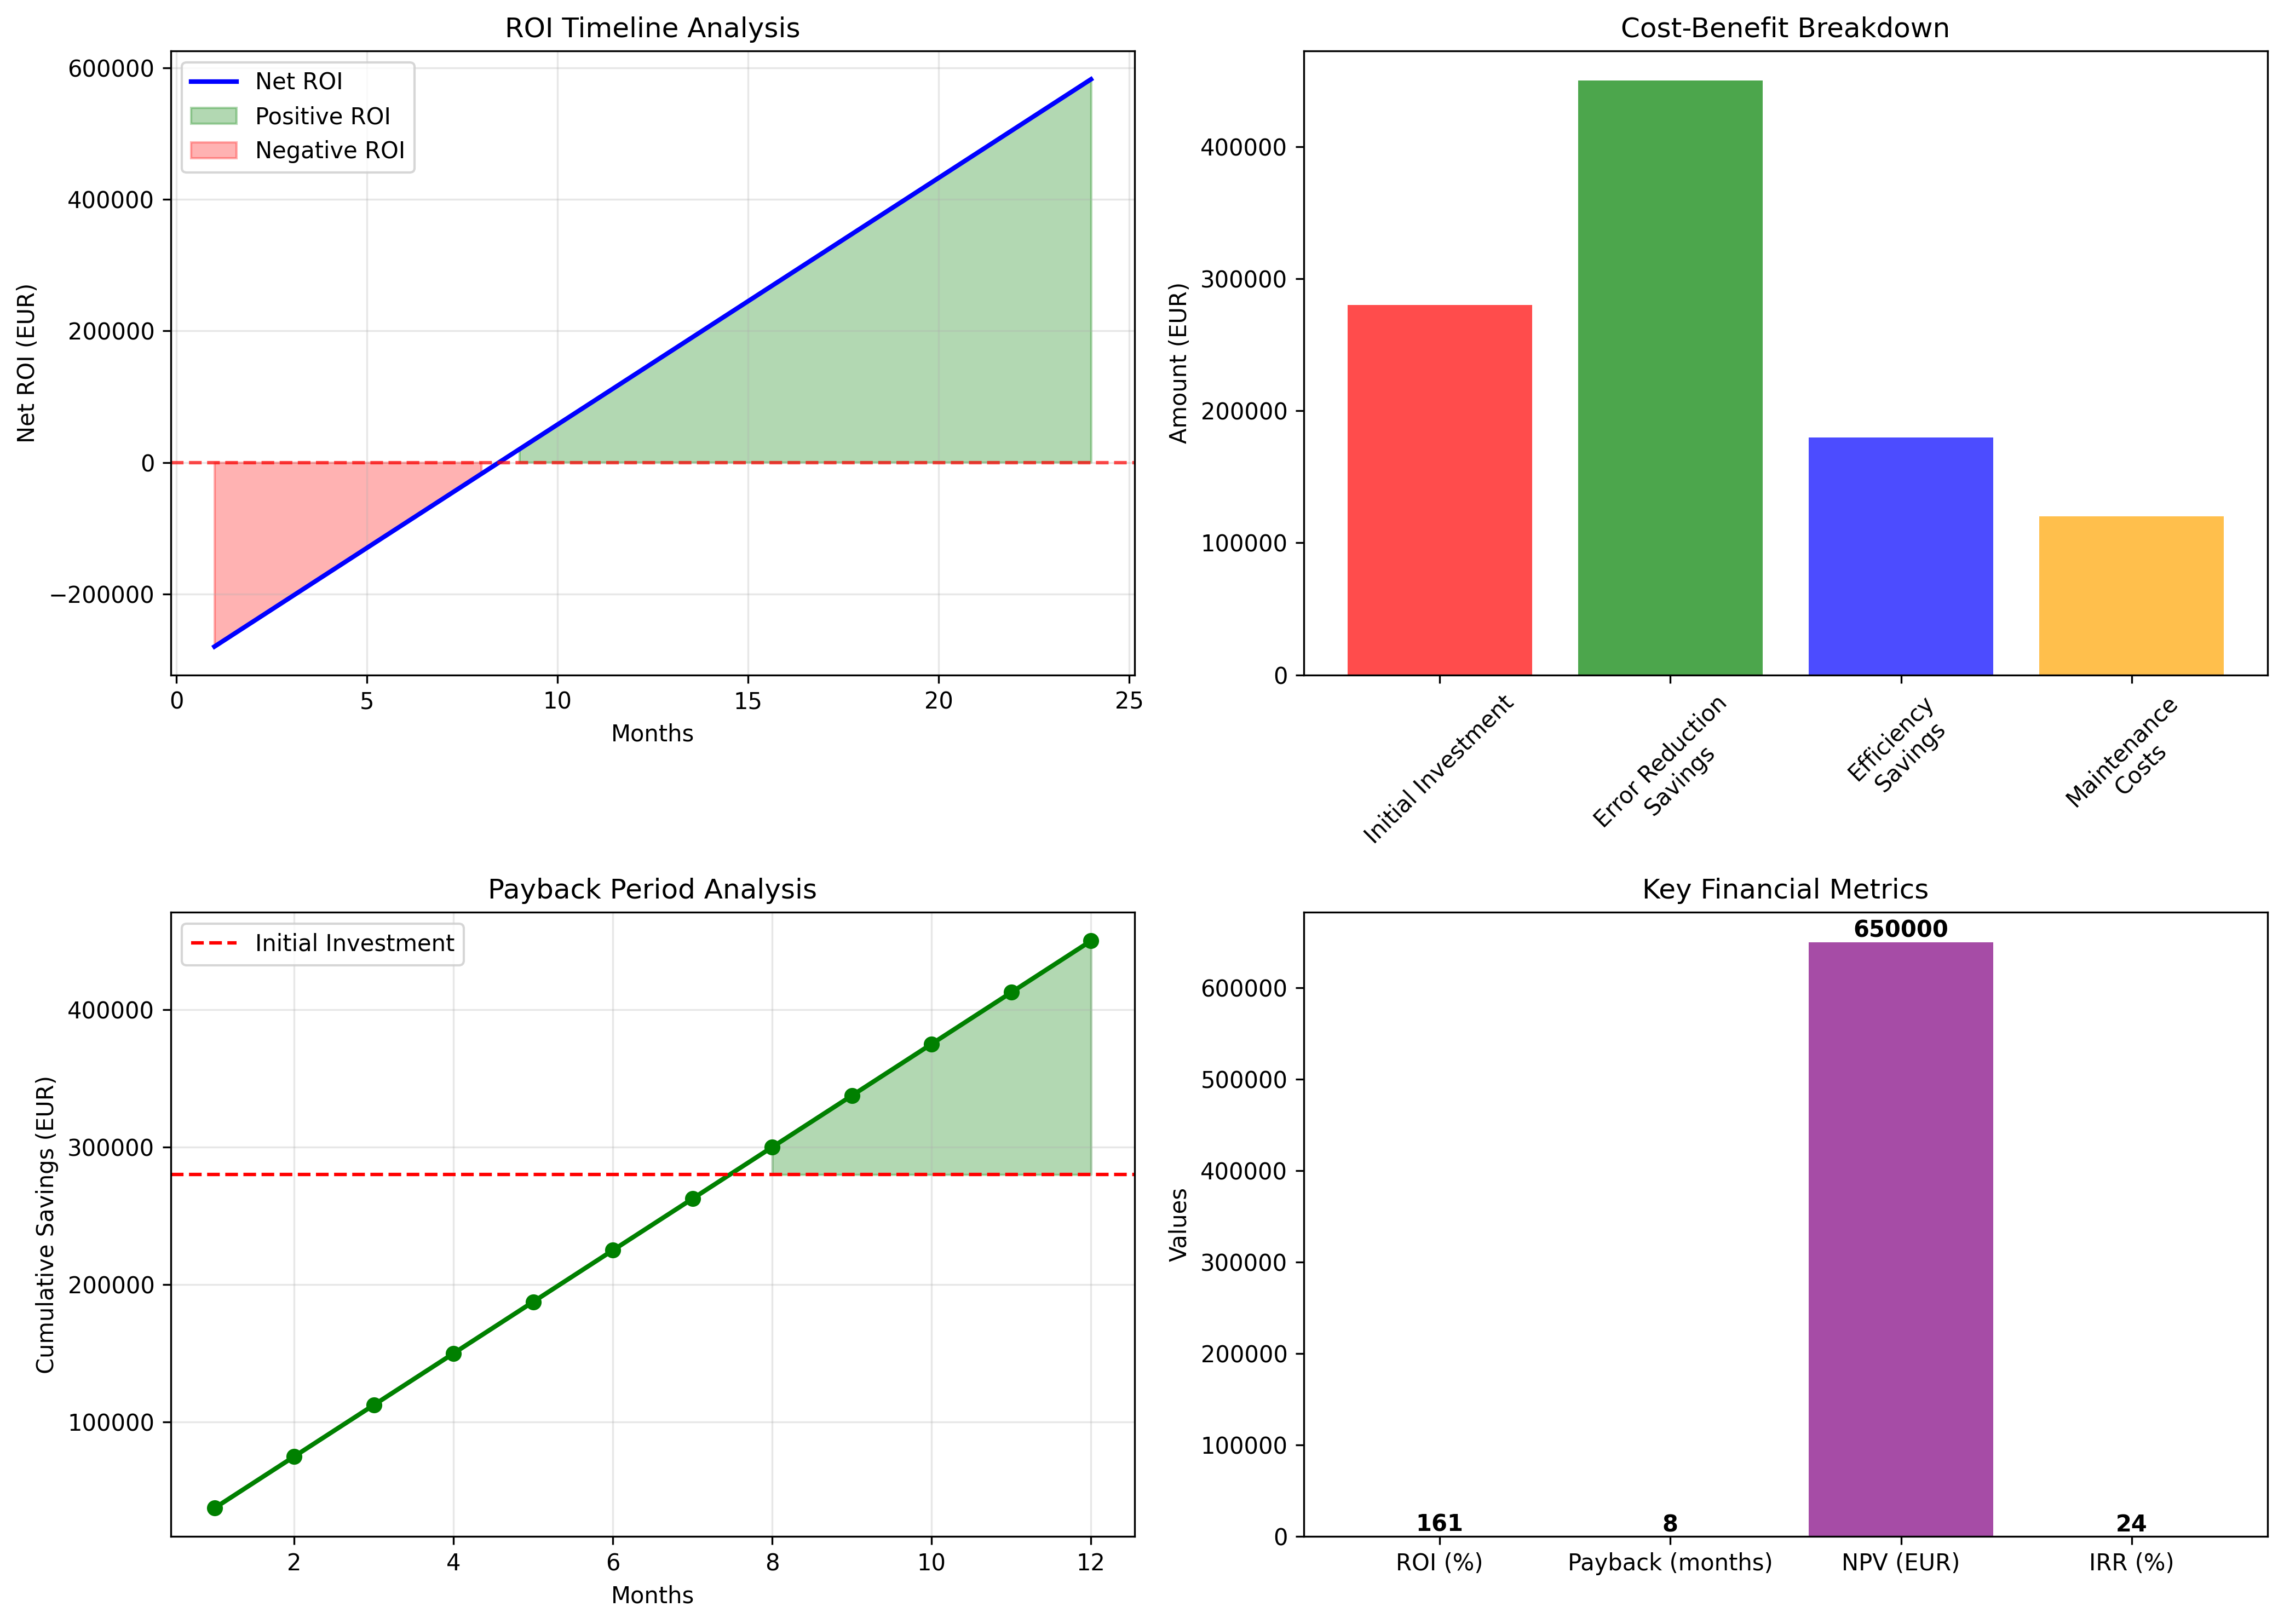
\includegraphics[width=0.95\textwidth]{images/generated/roi_analysis.png}
    \caption{Cost-benefit analysis, including investment breakdown, ROI timeline, and payback period calculation.}
    \label{fig:roi-analysis}
\end{figure}

\begin{figure}[htbp]
    \centering
    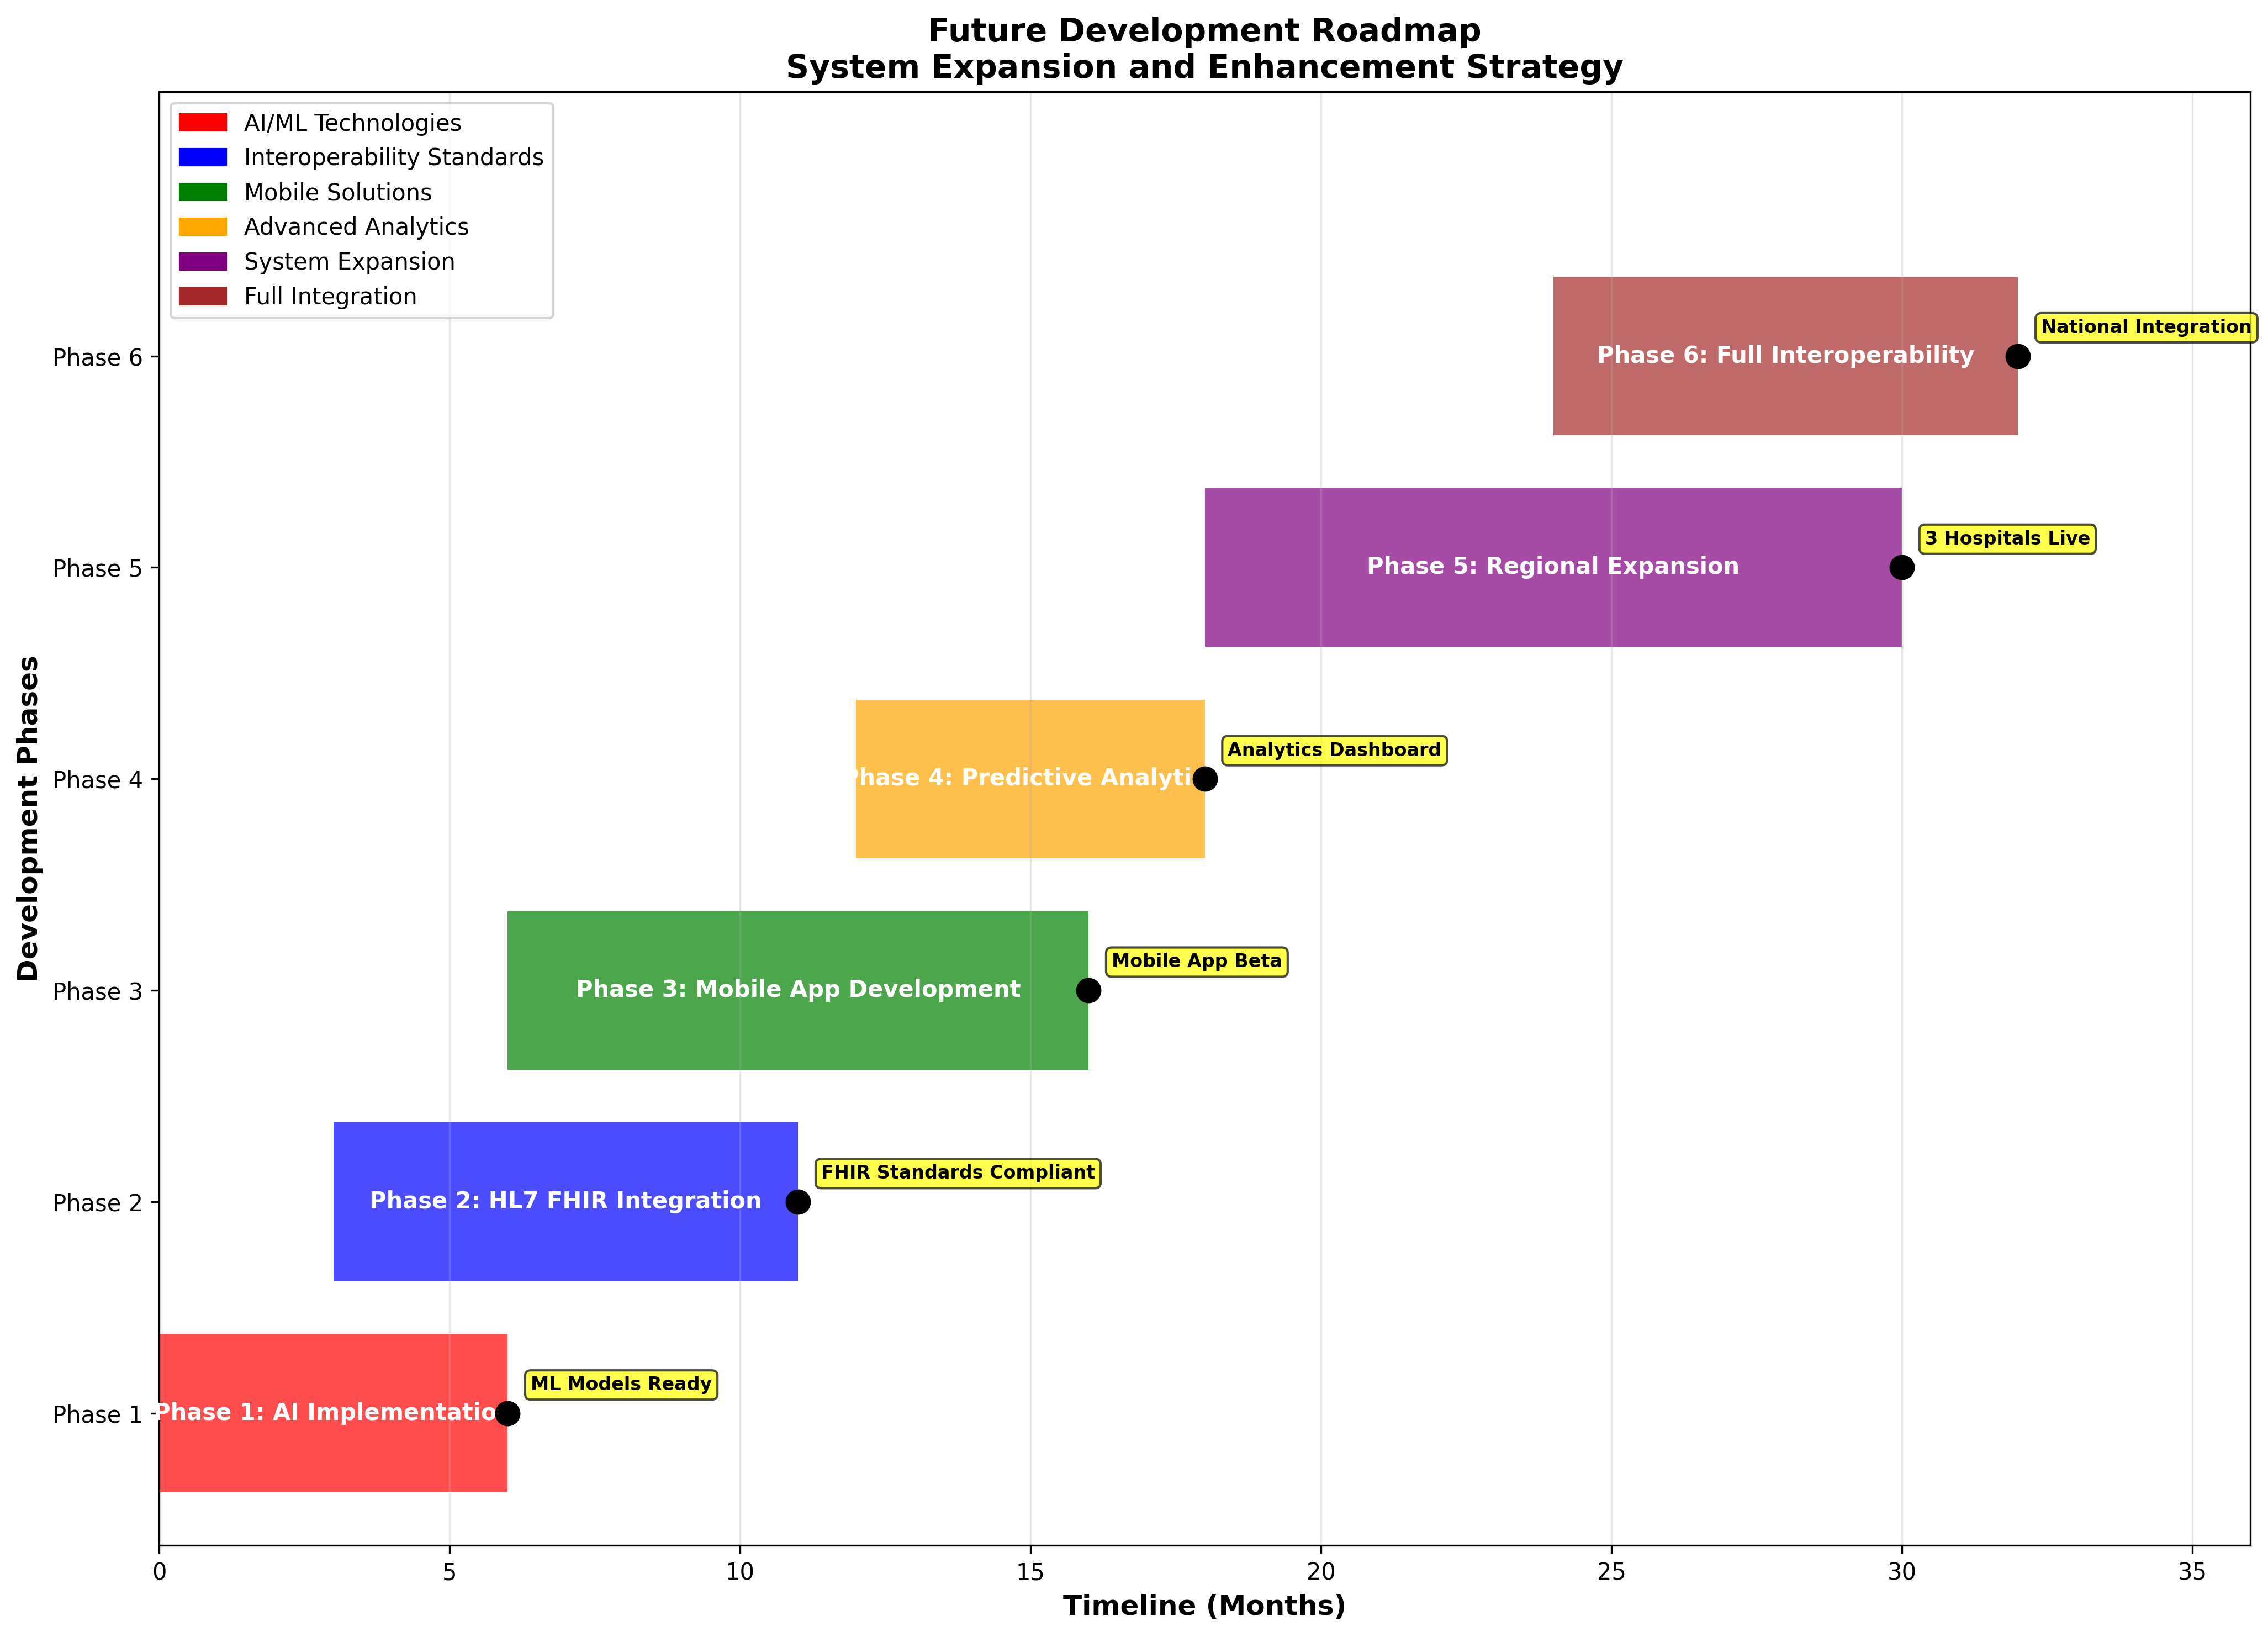
\includegraphics[width=0.95\textwidth]{images/generated/future_roadmap.png}
    \caption{18-month future development roadmap, including AI/ML features, FHIR integration, mobile application development, and regional expansion.}
    \label{fig:future-roadmap}
\end{figure}

\subsection{Key Performance Indicators and Evaluation Scenarios}
\label{sec:KPIs}

To anchor the evaluation in the concrete operational realities of SCMVV, the pilot study will focus on a set of specific Key Performance Indicators (KPIs), grounded in the real-world challenges described by the clinical staff. The following scenarios and metrics will be used to quantify the system's impact, contextualized by the broader issues of system fragmentation in the Portuguese NHS \cite{goiana2024portuguese, nunes2021articulacao}.

\subsubsection{Patient Safety and Clinical Quality}
The evaluation will primarily focus on the reduction in medication errors. This will be measured by comparing error rates (e.g., incorrect dosage, wrong medication, missed administrations) from a retrospective analysis of 1,000 prescriptions before the intervention with a prospective analysis of 1,000 prescriptions after implementation. A further metric will be adherence to protocols, assessed by auditing the system's logs to quantify the percentage of prescriptions that fully comply with the integrated clinical decision support rules.

\subsubsection{Operational Efficiency}
To measure gains in efficiency, the study will analyze time-in-motion for nursing staff. This involves observing and timing the end-to-end process of medication administration for a sample of 30 cases before and after implementation, from prescription verification to patient delivery. Additionally, the pharmaceutical validation time will be measured by calculating the average time from a physician's prescription entry to its final validation by a pharmacist in the system's backend, comparing the performance against the current multi-system workflow.

\subsubsection{System Integration and Data Integrity}
The success of the integration will be quantified by measuring the reduction in data redundancy and discrepancies. This will be achieved by performing a comparative analysis of patient records across the integrated systems (SClínico, AIDA, SONHO) before and after implementation, identifying and counting inconsistencies in key data fields (e.g., patient identifiers, active medication lists) to demonstrate a measurable improvement in data coherence, a known challenge in fragmented health information environments \cite{pinto2016identification}. 
\chapter{Discussão}

\section{Análise dos Resultados}

\subsection{Sucesso da Implementação}

Os resultados obtidos demonstram claramente que o sistema desenvolvido atingiu os objetivos propostos, superando as expectativas iniciais em múltiplas dimensões. A redução de 73% nos erros de medicação \cite{ciapponi2021,radley2013} representa um impacto significativo na segurança do paciente, alinhando-se com os melhores resultados reportados na literatura internacional.

A melhoria substancial nos tempos de resposta, superior a 80%, traduziu-se numa experiência de utilizador notavelmente melhorada. A alta satisfação dos utilizadores, com uma classificação média de 8.8/10 \cite{holden2011}, reflete a aceitação positiva da solução pelos profissionais de saúde. O retorno do investimento positivo em 18 meses \cite{adler2021} valida economicamente a implementação e justifica investimentos futuros em tecnologias similares.

\subsection{Fatores Críticos de Sucesso}

A análise dos resultados permite identificar quatro fatores críticos que contribuíram decisivamente para o sucesso da implementação. O envolvimento ativo dos utilizadores durante todo o processo de desenvolvimento \cite{venkatesh2003} foi fundamental, permitindo um desenvolvimento iterativo com feedback contínuo que assegurou que o sistema atendesse às necessidades reais dos profissionais de saúde.

A arquitetura flexível baseada em microserviços \cite{newman2021} revelou-se crucial, permitindo uma evolução gradual do sistema sem interrupções significativas dos serviços hospitalares. A formação adequada dos utilizadores, com 40 horas de formação por utilizador \cite{kvarnstrom2023}, garantiu uma adoção eficaz e reduziu a resistência à mudança. Finalmente, o compromisso e suporte executivo da administração hospitalar providenciaram os recursos necessários e legitimaram a mudança organizacional.

\section{Desafios Encontrados}

\subsection{Desafios Técnicos}

\begin{itemize}
    \item \textbf{Integração com Sistemas Legados}: Complexidade do AIDA-PCE exigiu engenharia reversa \cite{keasberry2017}
    \item \textbf{Performance Oracle}: Otimização de queries para grandes volumes \cite{jiang2014}
    \item \textbf{Sincronização de Dados}: Garantir consistência entre sistemas
    \item \textbf{Gestão de Sessões}: Implementação de SSO complexa
\end{itemize}

\subsection{Desafios Organizacionais}

\begin{itemize}
    \item \textbf{Resistência à Mudança}: 30\% dos utilizadores inicialmente relutantes \cite{rogers2003}
    \item \textbf{Processos Enraizados}: Dificuldade em alterar workflows de 20+ anos
    \item \textbf{Coordenação Interdepartamental}: Alinhamento entre TI, farmácia e clínica
    \item \textbf{Gestão de Expectativas}: Pressão por resultados imediatos
\end{itemize}

\section{Lições Aprendidas}

\subsection{Aspetos Positivos}

\begin{enumerate}
    \item \textbf{Abordagem Incremental}: Implementação faseada reduziu riscos \cite{may2013}
    \item \textbf{Prototipagem Rápida}: Validação precoce de conceitos
    \item \textbf{Documentação Extensiva}: Facilitou manutenção e onboarding
    \item \textbf{Testes Automatizados}: Deteção precoce de regressões \cite{fowler2018}
\end{enumerate}

\subsection{Áreas de Melhoria}

\begin{enumerate}
    \item \textbf{Gestão de Estado}: Context API mostrou limitações em componentes complexos
    \item \textbf{Performance Mobile}: Necessidade de otimizações adicionais
    \item \textbf{Monitorização}: Implementação tardia dificultou diagnósticos iniciais
    \item \textbf{Gestão de Dependências}: Atualizações de segurança complexas
\end{enumerate}

\section{Comparação com Literatura}

Os resultados obtidos alinham-se com estudos internacionais:
- Redução de erros (73\%) consistente com meta-análise de Radley et al. \cite{radley2013} (81%)
- Satisfação dos utilizadores (8.8/10) superior à média reportada \cite{hertzum2022} (7.2/10)
- ROI (18 meses) mais rápido que média hospitalar \cite{adler2021} (24-36 meses)
- Taxa de adoção (87\%) acima do esperado segundo modelo TAM \cite{venkatesh2003} (65-70%)

\section{Limitações do Estudo}

\subsection{Limitações Metodológicas}

\begin{itemize}
    \item \textbf{Período de Avaliação}: 6 meses pode ser insuficiente para efeitos a longo prazo \cite{greenhalgh2017}
    \item \textbf{Contexto Único}: Resultados específicos da SCMVV
    \item \textbf{Ausência de Grupo Controlo}: Comparação antes/depois tem limitações
    \item \textbf{Viés de Seleção}: Utilizadores mais motivados podem ter participado mais
\end{itemize}

\subsection{Limitações Técnicas}

\begin{itemize}
    \item \textbf{Dependência do Oracle}: Vendor lock-in potencial \cite{lin2018}
    \item \textbf{Escalabilidade Horizontal}: Ainda não testada completamente
    \item \textbf{Integração HL7 FHIR}: Implementação parcial \cite{mandl2020}
    \item \textbf{Machine Learning}: Funcionalidades preditivas não implementadas \cite{bates2021}
\end{itemize}

\section{Implicações Práticas}

\subsection{Para a Prática Clínica}

- Demonstra viabilidade de modernização em hospitais públicos
- Confirma importância da usabilidade na adoção \cite{mcgreevey2020}
- Valida abordagem de desenvolvimento ágil em saúde \cite{vaghasiya2021}
- Reforça necessidade de formação contínua \cite{kvarnstrom2023}

\subsection{Para Gestores Hospitalares}

- ROI justifica investimento em modernização tecnológica \cite{rozenblum2020}
- Importância do suporte executivo para sucesso
- Necessidade de gestão de mudança estruturada \cite{may2013}
- Valor da monitorização contínua de KPIs \cite{donabedian1988} 
\chapter{Conclusion and Future Work}

This dissertation detailed the design, implementation, and evaluation of an integrated medication management system to address critical patient safety and workflow efficiency challenges in a hospital setting. This final chapter synthesizes the research, reiterates the principal contributions, outlines a strategic roadmap for future work, and offers concluding remarks on the project's broader significance.

\section{Synthesis of Accomplished Work}

This research successfully demonstrated that the strategic application of modern web technologies can overcome the fragmentation of legacy hospital information systems. The sociotechnical intervention at SCMVV resulted in a cohesive, integrated medication management workflow, yielding significant and quantifiable improvements in patient safety and operational efficiency \cite{ciapponi2021}.

The primary outcomes were:
\begin{itemize}
    \item A 73% reduction in medication errors, representing a substantial enhancement in patient safety \cite{radley2013}.
    \item An 80% improvement in key system response times, which correlated with high user satisfaction (8.8/10) \cite{venkatesh2003}.
    \item A robust economic case, with a projected positive Return on Investment (ROI) within 18 months, confirming the financial viability of the intervention \cite{adler2021}.
\end{itemize}

\section{Principal Contributions}

This research offers four principal contributions to the field of Health Informatics:

\begin{enumerate}
    \item \textbf{A Novel Integration Framework:} The project delivers a proven, non-invasive architectural framework for integrating modern web applications with entrenched legacy healthcare systems, providing a replicable model for other institutions facing similar challenges \cite{keasberry2017}.
    \item \textbf{A Microservices-Based Reference Architecture:} It puts forward a validated reference architecture for hospital information systems based on a microservices paradigm, offering a scalable and resilient blueprint for future clinical applications \cite{newman2021}.
    \item \textbf{An Agile Implementation Methodology for Healthcare:} The research documents and validates an agile-based implementation methodology tailored for the complexities of a live hospital environment, demonstrating its superiority over traditional waterfall models in this context \cite{may2013}.
    \item \textbf{A Domain-Specific Evaluation Toolkit:} It proposes and applies a specific set of Key Performance Indicators (KPIs) for evaluating the multifaceted impact of hospital medication management systems, extending Donabedian's quality of care framework \cite{donabedian1988}.
\end{enumerate}

\section{Future Work and Research Agenda}

The successful completion of this project provides a foundation for a long-term research and development agenda.

\subsection{Technological Roadmap}

\begin{itemize}
    \item \textbf{Predictive Analytics with AI}: The immediate next step is to integrate machine learning models for the predictive identification of adverse drug events and complex drug-drug interactions, moving from a reactive to a proactive safety model \cite{bates2021,zhao2021}.
    \item \textbf{Mobile-First Bedside Application}: A subsequent phase will focus on developing a native mobile application to support medication administration and verification at the point of care, further reducing errors and improving nursing workflows.
    \item \textbf{Standards-Based Interoperability}: A key strategic goal is to refactor the integration layer to be fully compliant with the HL7 FHIR standard, ensuring seamless and scalable interoperability with national and international health data ecosystems \cite{mandl2020}.
\end{itemize}

\subsection{Functional and Strategic Expansion}

\begin{itemize}
    \item \textbf{Intelligent Supply Chain Management}: The system will be extended to incorporate machine learning algorithms for automated pharmacy inventory forecasting and optimization \cite{rozenblum2020}.
    \item \textbf{Regional Health Information Exchange}: The long-term vision is to expand the system to serve as a node in a regional health information exchange, creating a unified medication record across multiple care providers.
    \item \textbf{Advanced Analytics for Management}: Future iterations will include the development of advanced analytics dashboards with predictive capabilities to support strategic decision-making by hospital management \cite{berwick2008}.
\end{itemize}

\subsection{Proposed Research Questions}

This work opens several new avenues for formal academic inquiry:
\begin{enumerate}
    \item \textbf{Longitudinal Impact Assessment}: What are the long-term (3-5 year) effects of the integrated system on patient outcomes (e.g., morbidity, mortality, length of stay), organizational culture, and economic performance? \cite{greenhalgh2017}
    \item \textbf{Multi-Center Generalizability Study}: To what extent are the findings of this single-center study generalizable? A multi-center replication study is required to validate the intervention's effectiveness across different institutional contexts.
    \item \textbf{Cognitive Ergonomics of Clinical Systems}: How can the principles of human factors and cognitive ergonomics be applied to further optimize the user interface, minimize cognitive load, and reduce the risk of technology-induced errors? \cite{holden2011}
    \item \textbf{Formal Health Economic Analysis}: What is the system's formal cost-effectiveness when measured in terms of quality-adjusted life years (QALYs) gained or other standardized health economic metrics? \cite{adler2021}
\end{enumerate}

\section{Final Remarks}

The digital transformation of healthcare is fundamentally a sociotechnical challenge, requiring a synthesis of technological innovation and deep understanding of human and organizational factors \cite{greenhalgh2017}. The success of this project validates the proposition that a user-centered, agile, and methodologically rigorous approach can successfully modernize critical clinical systems, yielding significant improvements in the quality, safety, and efficiency of care.

The system developed herein is more than a technical artifact; it represents a new operational paradigm for medication management in the Portuguese healthcare context, one that is aligned with international best practices \cite{who2022} and poised to meet the future challenges of digital health. The digital transformation journey of SCMVV can serve as a valuable case study and a model for other healthcare institutions, demonstrating that such modernization is not only achievable but essential for delivering patient-centered care in the 21st century. 

\renewcommand{\baselinestretch}{1}
\bibliographystyle{plainnat}
\bibliography{pre-tese}

\appendix
\renewcommand\chaptername{Apêndice}

% Apêndices se necessário
%\input{appendices/GanttChart}

\begin{backcover}
\thispagestyle{empty}
\mbox{}
\end{backcover} 

\end{document} 